\chapter{Metodología}
\label{ch:metodologia}

A lo largo de este capítulo señalaremos con qué métodos y herramientas lograremos, con éxito, el objetivo de este trabajo. Estas estarán basadas en la experiencia de trabajos previos revisados en el Capitulo~\ref{ch:marcoteorico} y metodologías ampliamente utilizadas en la minería de datos [cita] para la obtención de información valiosa en los datos de forma efectiva.

\section{Minería de Datos}
La cantidad de datos ha ido aumentando de forma exponencial debido a los avances en la tecnología de la computación necesitando que la búsqueda de conocimiento sea de forma automatizada.

La minería de datos es un proceso que se ideó pensando en descubrir información valiosa dentro de una gran cantidad de datos\footnote{Para este trabajo definimos datos como información textual o numérica con alguna estructura dada} como flujo de entrada y nos entrega conocimiento.\footnote{Esto es una analogía a la industria de la minería donde se extrae los minerales rocosos donde una parte de esta es valiosa}

La minería de datos, tal como es posible observar en la Figura\ref{fig:datamining}, tiene como finalidad generar conocimiento  valioso a partir de un conjunto de datos, la que luego es utilizada para la toma de decisiones o para la comprensión de un fenómeno, y se realiza a través de diferentes tareas que se pueden realizar con los diferentes algoritmos disponibles que los señalaremos posteriormente.

\begin{figure}[H]
  \centering
    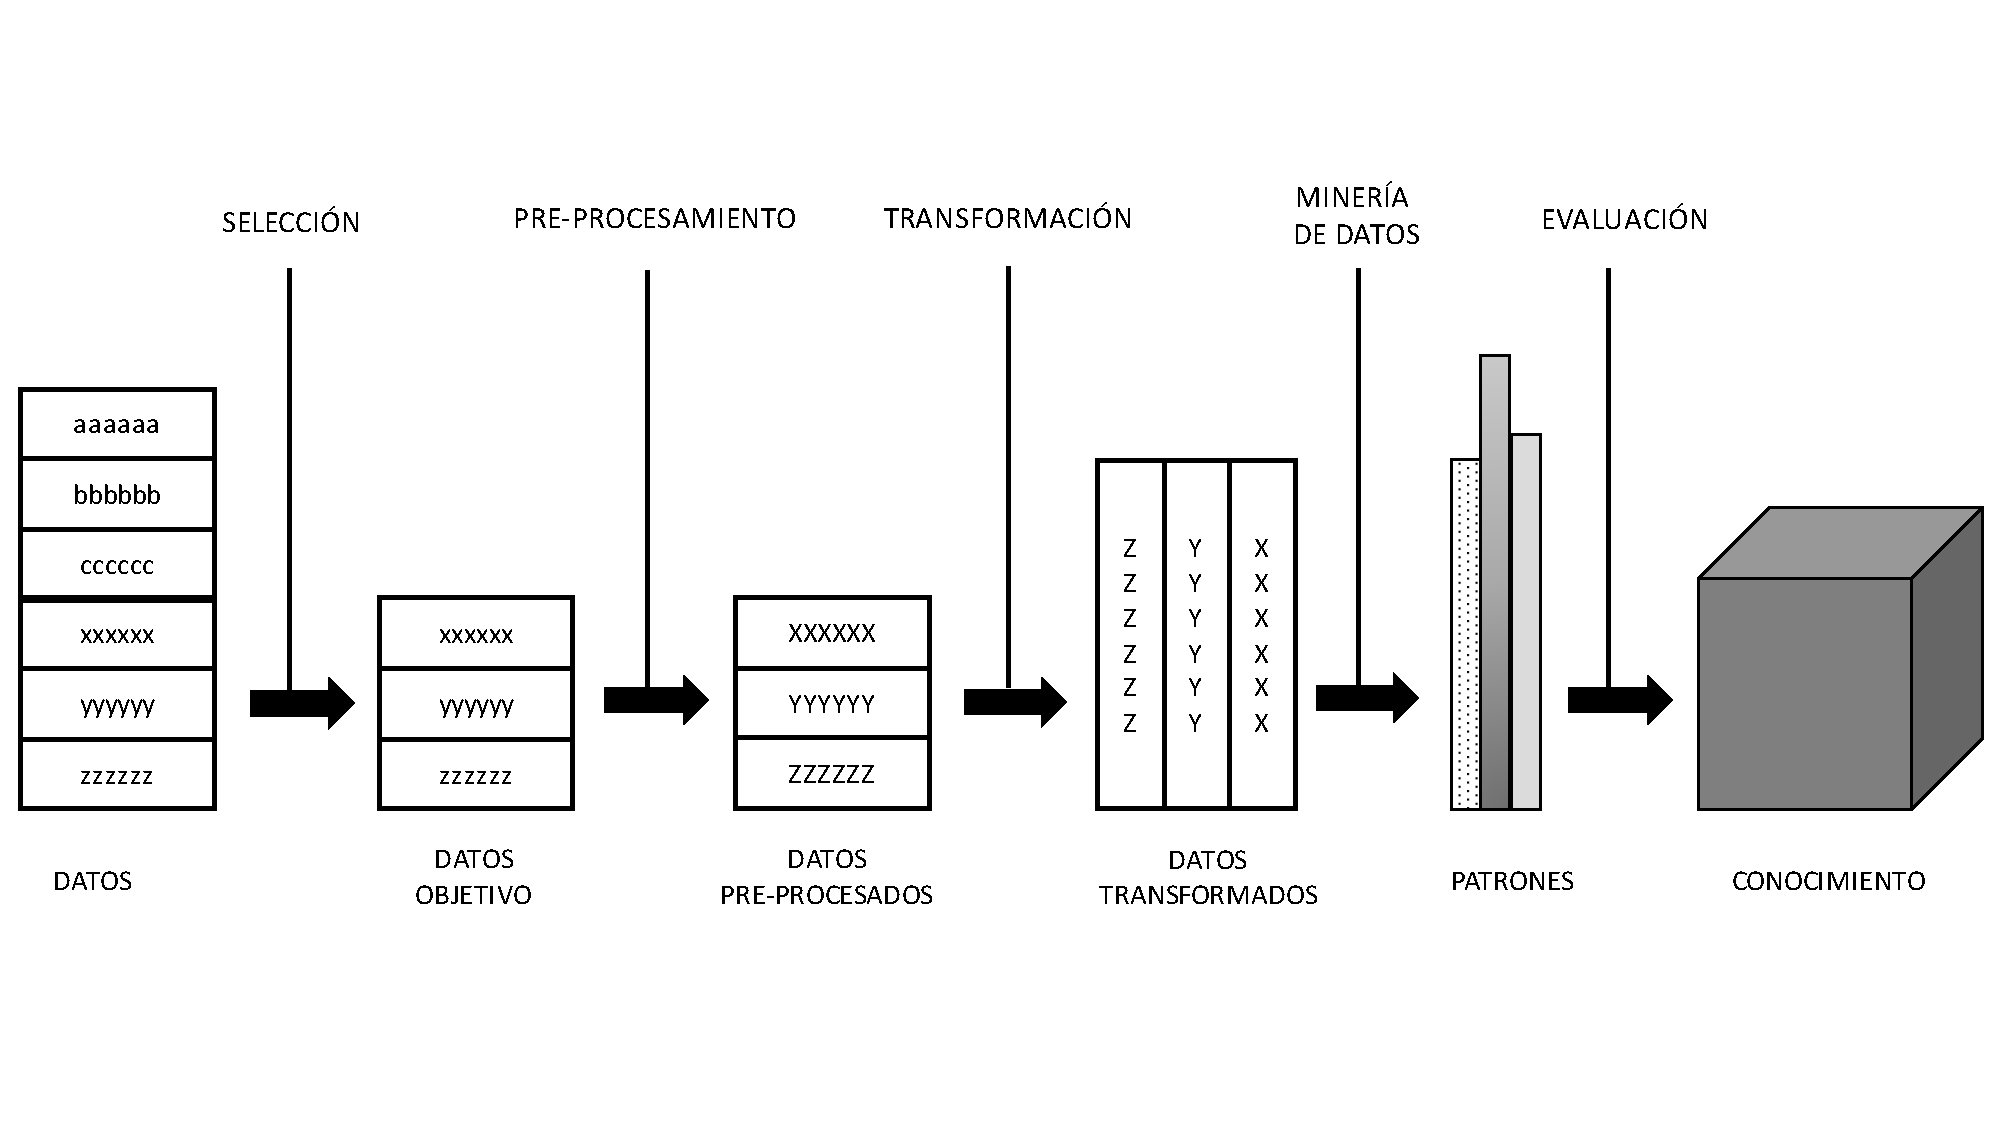
\includegraphics[width=0.9\textwidth]{Figuras/DM}
      \caption{Proceso de Minería de Datos.}
    \label{fig:datamining}
\end{figure}

%http://storm.cis.fordham.edu/~gweiss/papers/data-mining-chapter-2010.pdf

Para realizar minería de datos se han establecido diferentes metodologías para asegurar un resultado coherente con lo que se busca obtener. Existen diferentes metodologías que serán mencionadas y descritas brevemente a continuación.

\subsection{KDD}

%[cita] http://www.csd.uwo.ca/faculty/ling/cs435/fayyad.pdf

La metodología \textit{Knowledge Discovery in Databases} o Proceso de Extracción del Conocimiento, tal como su nombre lo dice, es un proceso no trivial de descubrimiento de conocimiento e información potencialmente útil dentro de los datos contenidos en algún repositorio de información (cita de Han, J.; Kamber M. (2001). Data Mining: Concepts ans Techniques. Morgan Kaufmann Publishers, USA.). 

Es un proceso iterativo que explora de forma exhaustiva altos volúmenes de datos con el fin de determinar relaciones. De esta manera es posible extraer información de calidad que se puede utilizar para generar modelos con los datos. 

\begin{figure}[H]
  \centering
    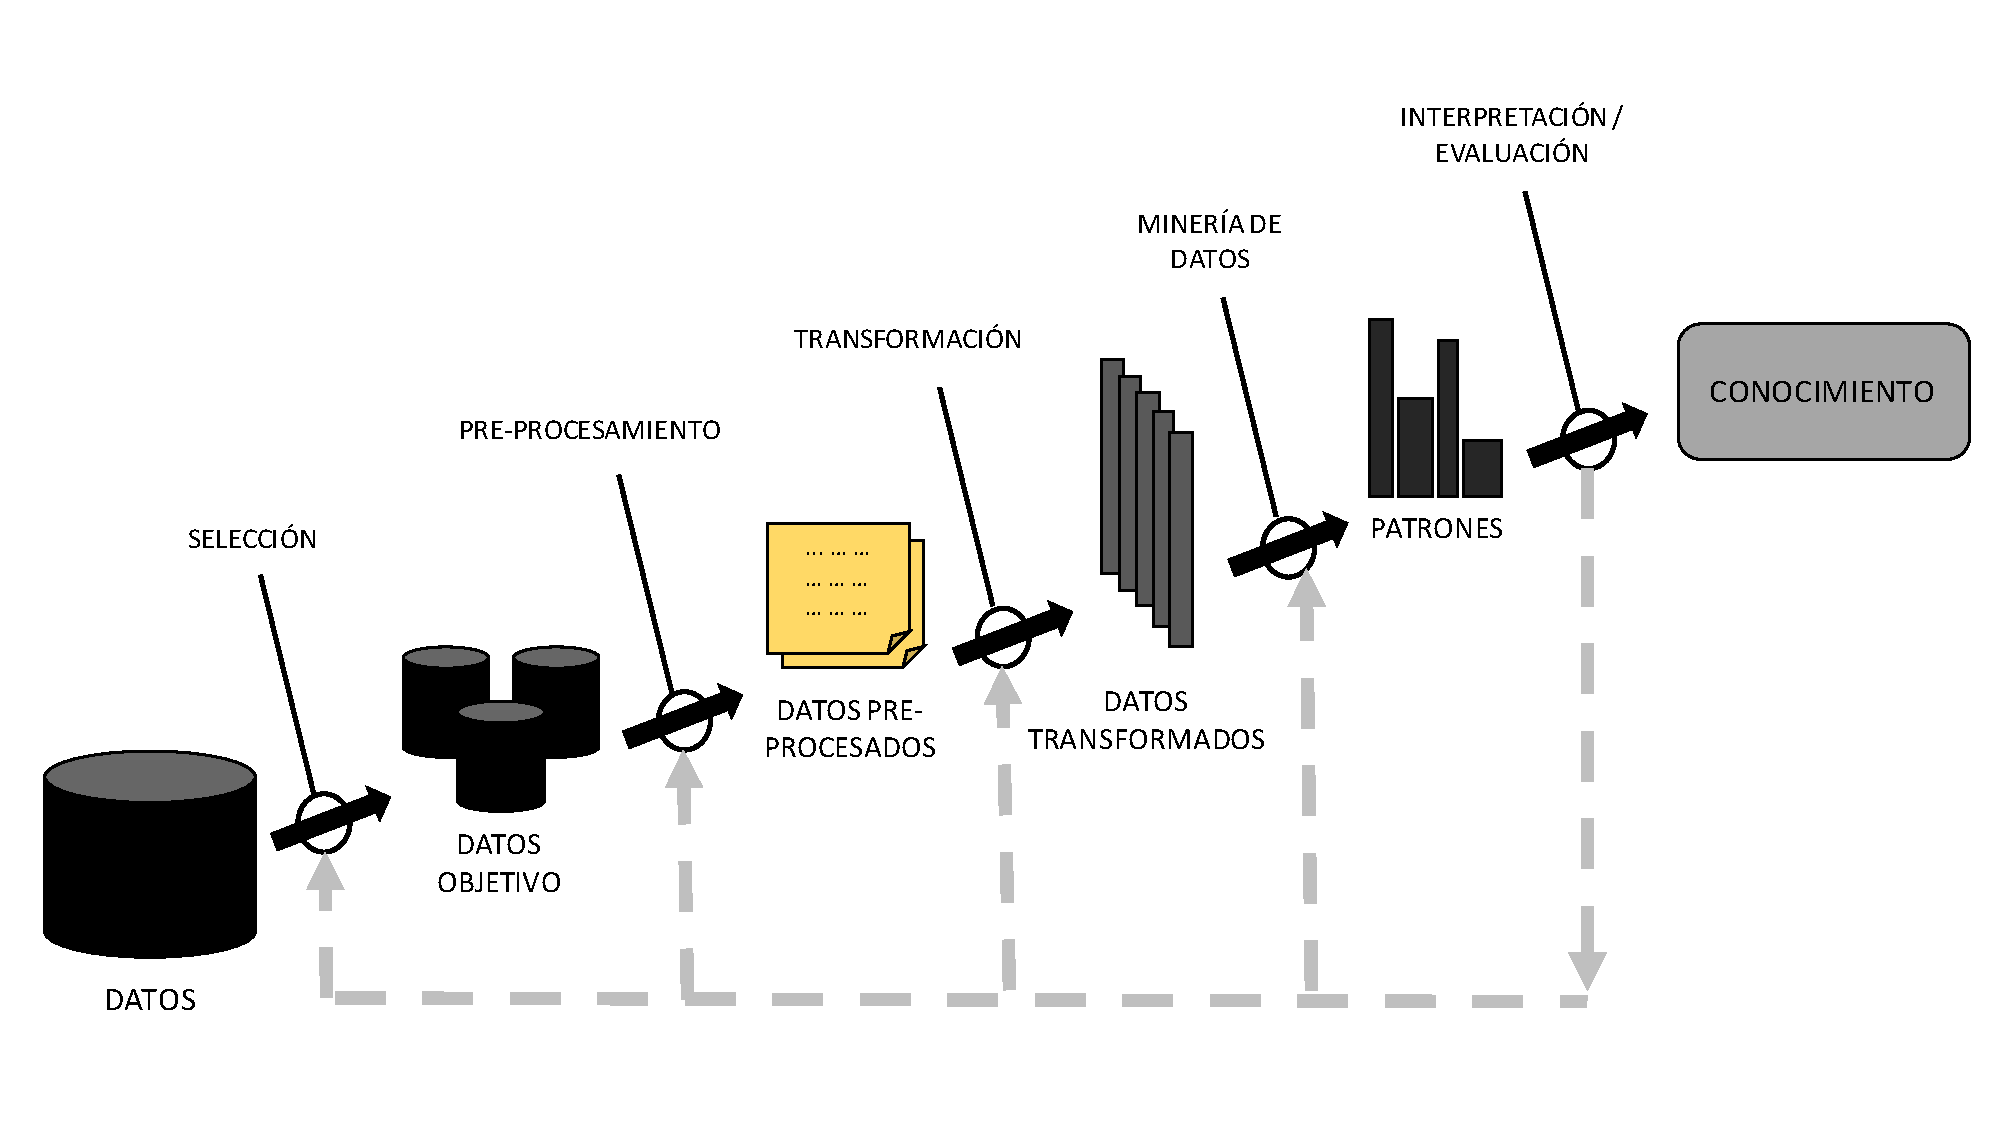
\includegraphics[width=0.9\textwidth]{Figuras/KDD}
      \caption{Etapas de la metodología KDD.}
    \label{fig:kdd}
\end{figure}

Como muestra la Figura~\ref{fig:kdd}, el proceso de extracción del conocimiento consta de cinco etapas:
\begin{description}
  \item[1. Selección de Datos:] se determinan las fuentes de datos y el tipo de información a utilizar, es cuando los datos relevantes para el análisis son extraídos de la o las fuentes de datos.
  \item[2. Pre-Procesamiento:] se procede a preparar y limpiar los datos extraídos desde las distintas fuentes de datos seleccionadas anteriormente. Este paso es fundamental para las fases posteriores.Para manejar datos faltantes, inconsistentes o que estén fuera de rango se utilizan diversas estrategias con el fin de obtener una estructura de datos adecuada para su posterior transformación.
  \item[3. Transformación:] consiste en el tratamiento preliminar de los datos, transformando y generando nuevas variables con una estructura de datos apropiada a partir de las ya existentes. Se realizan operaciones de agregación o normalización, consolidando los datos de una forma necesaria para la fase siguiente. 
  \item[4. Minería de Datos:] consiste en el modelamiento propiamente tal, para lo que se aplican métodos inteligentes con el fin de extraer patrones desconocidos, válidos, nuevos, potencialmente útiles y comprensibles y que están "ocultos" en los datos.
  \item[5. Interpretación y Evaluación:] finalmente se identifican los patrones obtenidos y que son realmente interesantes, además de evaluar los resultados obtenidos.
\end{description}

\subsection{SEMMA}
La metodología SEMMA, acrónimo de \textit{Sample, Explore, Modify, Model, Assess}, se define como un proceso de selección, exploración y modelamiento de grandes cantidades de datos para descubrir patrones de negocios desconocidos. 

\begin{figure}[H]
  \centering
    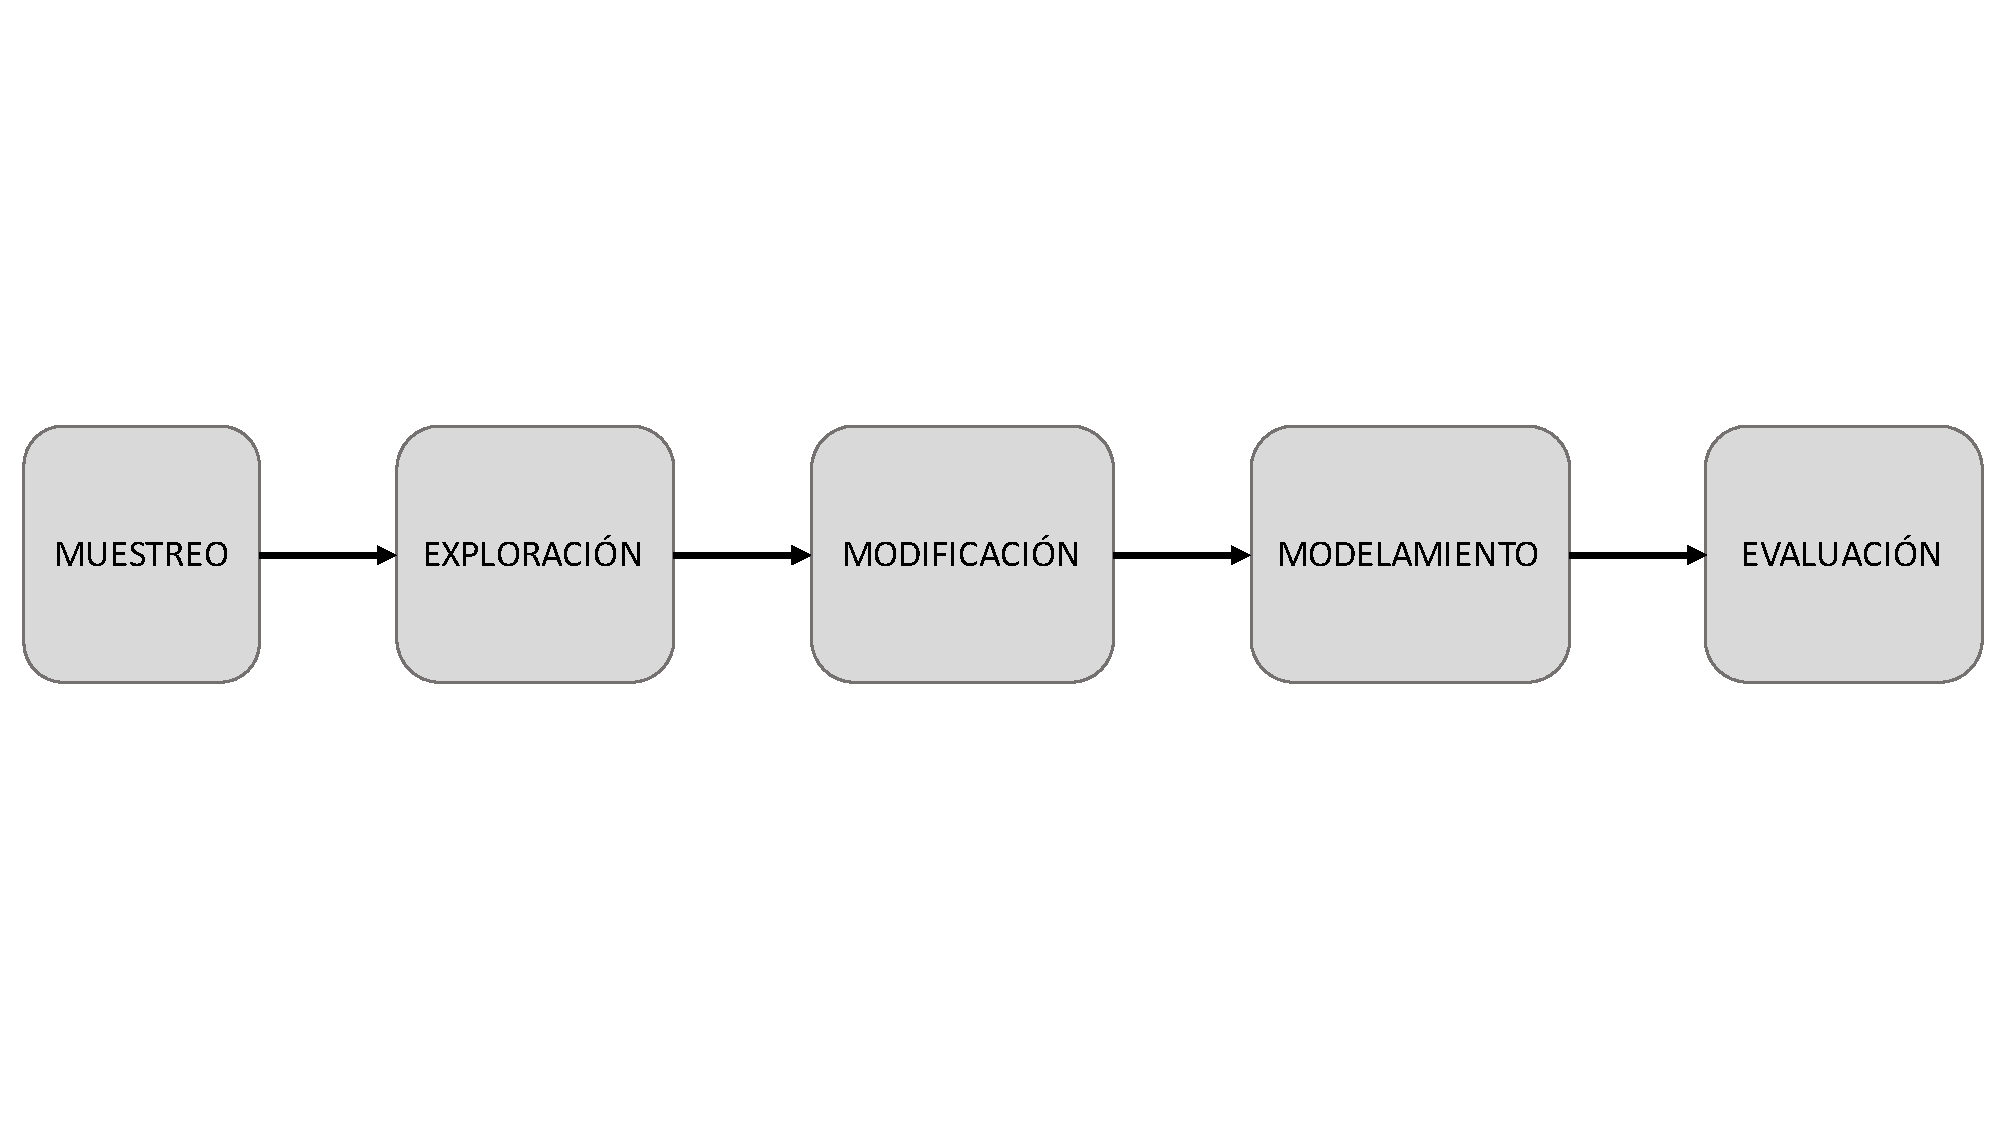
\includegraphics[width=0.9\textwidth]{Figuras/SEMMA}
      \caption{Etapas de la metodología SEMMA.}
    \label{fig:semma}
\end{figure}

En la Figura~\ref{fig:semma} es posible observar que esta metodología consta de cinco etapas:
\begin{description}
  \item[1. Muestreo:] es la etapa inicial, en la cual se procede a preparar los datos para su posterior exploración. En esta etapa es común la utilización del nodo de partición (especialmente si se quiere realizar árboles de decisión o redes neuronales). 
  \item[2. Exploración:] en esta etapa, como lo dice su nombre, se procede a explorar los datos, por lo que es una de las más trabajosas. Se tiene un nodo que permite explorar gráficamente los datos y otro de selección de variables que permite eliminar aquellos datos de entrada que no tienen relación con la variable objetivo, inclusive se puede realizar un análisis de conglomerados o una segmentación.
  \item[3. Modificación:] en esta etapa el foco es la selección y transformación de variables y datos que servirán para la posterior construcción de modelos. Entre otras tareas, destaca la reducción de dimensión y la imputación de datos perdidos o anómalos.
  \item[4. Modelamiento:] en esta etapa se procede a la selección de modelos. Esta elección depende esencialmente de los datos y variables que se tienen, y de obtener modelos fácilmente entendibles. Entre los modelos está la regresión, la regresión logística, árboles de decisión, análisis factorial discriminante, redes neuronales, entre otros. Se puede aplicar más de uno a la vez, para luego comparar los resultados obtenidos.
  \item[5. Evaluación:] etapa final en la cual se procede a comparar los modelos aplicados y los resultados que se obtienen de ellos. 
\end{description}
[cita]

\subsection{CRISP-DM}
La metodología CRISP-DM o \textit{Cross-Industry Standard Process for Data Mining} es un estándar para los proyectos de minería de datos que incluye un modelo y una guía, estructurados en fases que pueden ser bidireccionales, es decir, al desarrollar una fase es posible revisar parcial o totalmente las anteriores. 

\begin{figure}[H]
  \centering
    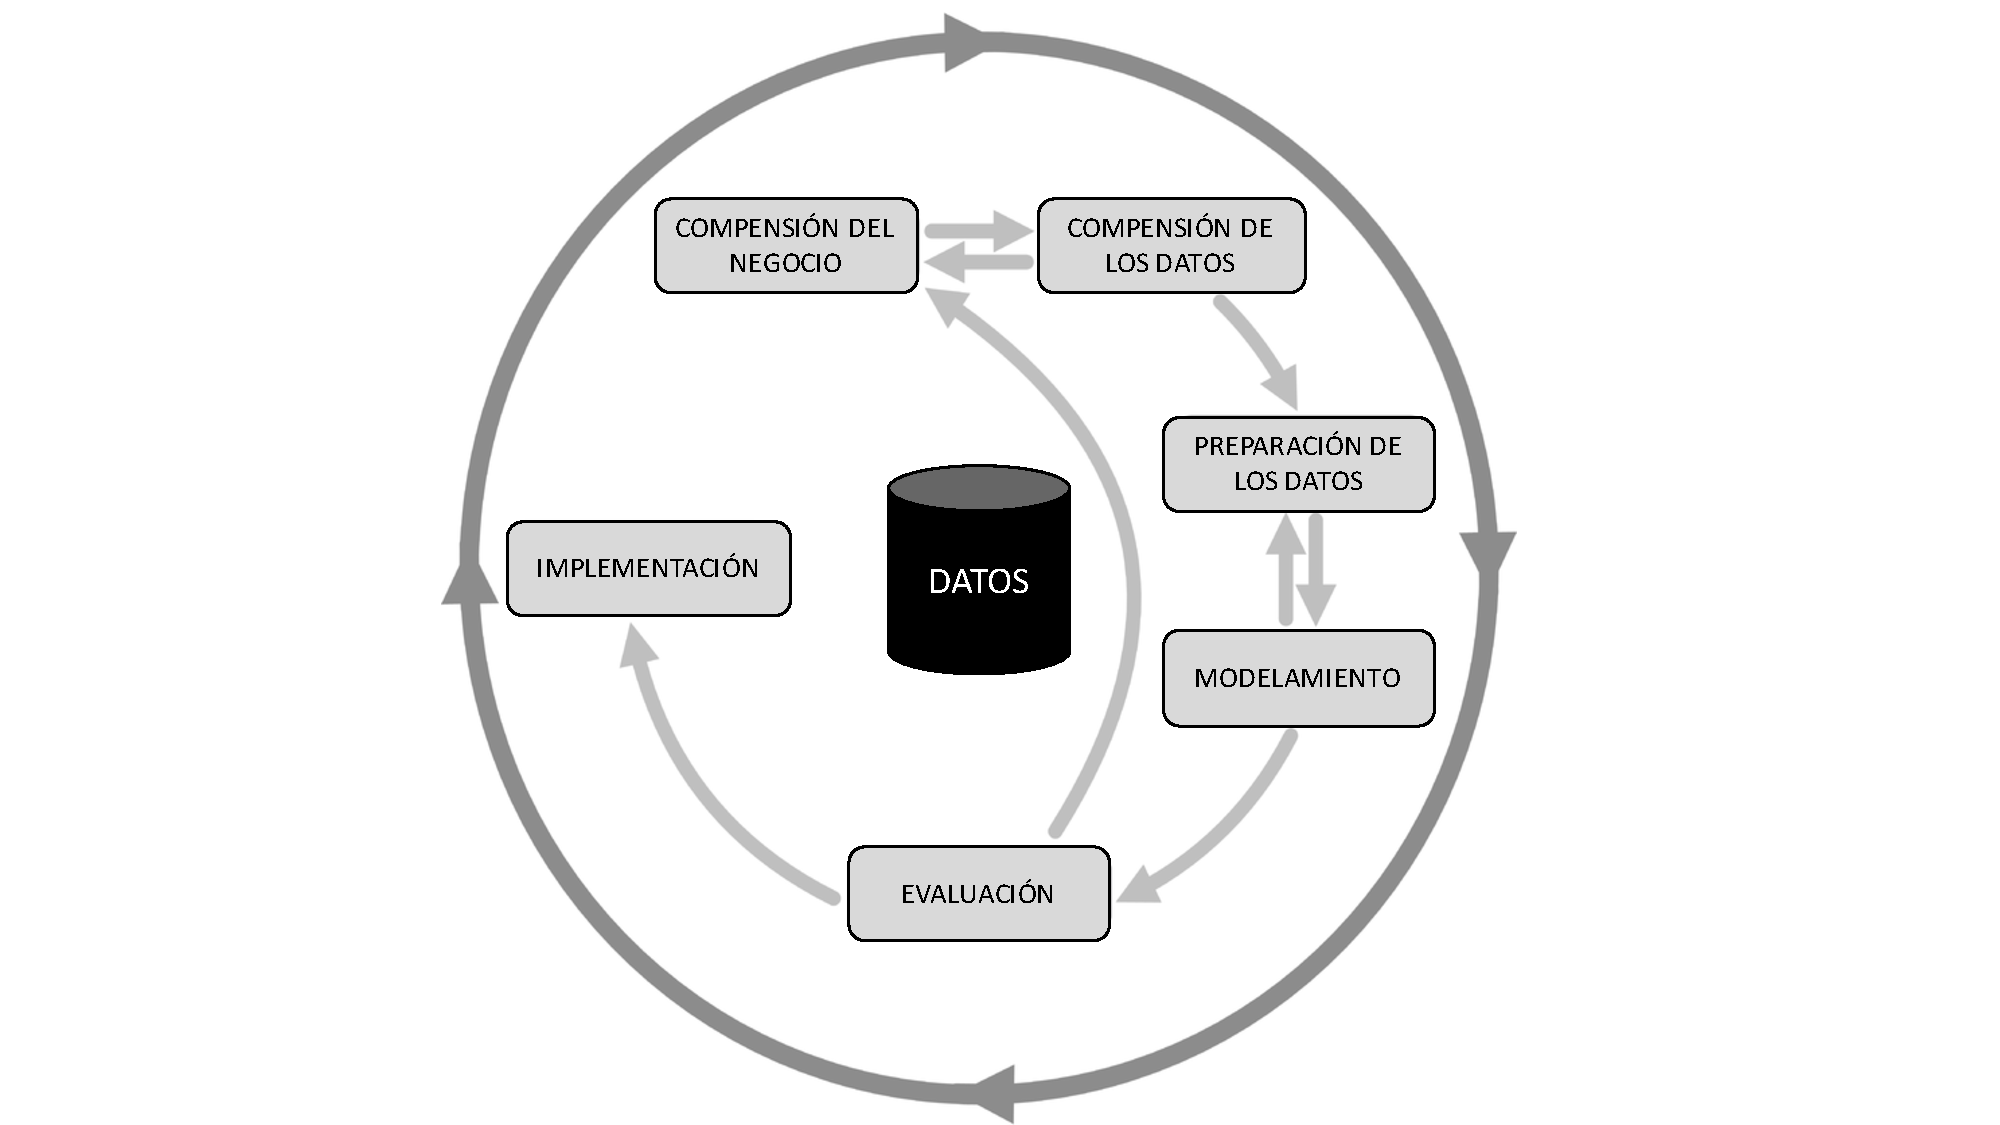
\includegraphics[width=0.99\textwidth]{Figuras/CRISP}
      \caption{Etapas de la metodología CRISP-DM.}
    \label{fig:crisp}
\end{figure}

Como es posible observar en la Figura~\ref{fig:crisp}, esta metodología estructura el proceso en seis fases cuya sucesión no es necesariamente rígida. Cada fase se descompone en varias tareas generales de segundo nivel. Las tareas generales se proyectan a tareas específicas, pero en ningún momento se propone como realizarlas. Es decir, CRISP-DM establece un conjunto de tareas y actividades para cada fase del proyecto pero no especifica cómo llevarlas a cabo.

Las fases son: 
\begin{description}
  \item[1. Comprensión del Negocio:] fase inicial cuyo objetivo es la comprensión de los objetivos y requisitos del cliente, para luego convertir este conocimiento en objetivos técnicos y en un plan de proyecto. 
  \item[2. Comprensión de los Datos:] el objetivo es establecer un primer contacto con el problema, por lo que requiere una recolección inicial de datos para familiarizarse con ellos, identificar su calidad y establecer las relaciones más evidentes para luego definir las primeras hipótesis. Esta fase junto a las próximas dos, son las que demandan el mayor esfuerzo y tiempo en un proyecto de minería de datos.
  \item[3. Preparación de los Datos:] una vez efectuada la recolección inicial de datos, se procede a su preparación para adaptarlos a las técnicas de minería de datos que posteriormente se utilicen. Este proceso incluye tareas generales de selección de datos a los que se va a aplicar una determinada técnica de modelado, limpieza de datos, generación de variables adicionales, integración de diferentes orígenes de datos y cambios de formato.
  \item[4. Modelamiento:] se seleccionan las técnicas de modelado apropiadas para el proyecto. Esta selección se debe realizar en función de los siguientes criterios: que sea apropiada al problema, disponer de los datos adecuados, cumplir con los requisitos del problema, tiempo adecuado para obtener un modelo y conocimiento de la técnica. 
  \item[5. Evaluación:] se procede a la evaluación del modelo considerando el cumplimiento de los criterios de éxito del problema. Además, debe considerarse que la fiabilidad calculada para el modelo se aplique sólo para los datos sobre los que se realizó el análisis. Es preciso revisar el proceso, teniendo en cuenta los resultados obtenidos, para poder repetir algún paso anterior, en el que se haya posiblemente cometido algún error. Es importante considerar que se pueden emplear múltiples herramientas para la interpretación de los resultados. Luego, si el modelo generado es válido en función de los criterios de éxito establecidos en la fase anterior, se procede a la explotación del modelo.
  \item[6. Implementación:] luego de que el modelo ha sido construido y validado, se procede a transformar el conocimiento obtenido en acciones dentro del proceso de negocio.
\end{description}

[cita] 
%http://oldemarrodriguez.com/yahoo_site_admin/assets/docs/Documento_CRISP-DM.2385037.pdf

\subsection{Selección de una metodología}

Para poder cumplir con los objetivos del trabajo debemos seleccionar una metodología de minería de datos. Los estudios muestran que la metodología CRISP-DM es la más simple y a la vez completa, abarcando desde el entendimiento del negocio hasta la implementación de la herramienta de minería de datos.[cita]A Comparative Study of Data Mining Process Models (KDD, CRISP-DM and SEMMA) Además, se ha visto durante varios años que la metodología CRISP-DM es la más utilizada dentro de la comunidad [cita] http://www.kdnuggets.com/2014/10/crisp-dm-top-methodology-analytics-data-mining-data-science-projects.html

% Please add the following required packages to your document preamble:
% \usepackage{multirow}
% \usepackage{graphicx}
% \usepackage[table,xcdraw]{xcolor}
% If you use beamer only pass "xcolor=table" option, i.e. \documentclass[xcolor=table]{beamer}
\begin{table}[H]
\centering
\resizebox{\textwidth}{!}{%
\begin{tabular}{|c|c|c|c|}
\hline
\rowcolor[HTML]{C0C0C0} 
{\color[HTML]{000000} \textbf{\begin{tabular}[c]{@{}c@{}}Modelos de Procesos de\\ Minería de Datos\end{tabular}}} & {\color[HTML]{000000} \textbf{KDD}} & {\color[HTML]{000000} \textbf{CRISP-DM}} & {\color[HTML]{000000} \textbf{SEMMA}} \\ \hline
{\color[HTML]{000000} Número de pasos} & {\color[HTML]{000000} 9} & {\color[HTML]{000000} 6} & {\color[HTML]{000000} 5} \\ \hline
{\color[HTML]{000000} } & {\color[HTML]{000000} \begin{tabular}[c]{@{}c@{}}Desarrollo y comprensión \\ de la aplicación\end{tabular}} & {\color[HTML]{000000} Entendimiento del negocio} & {\color[HTML]{000000} ------} \\ \cline{2-4} 
{\color[HTML]{000000} } & {\color[HTML]{000000} \begin{tabular}[c]{@{}c@{}}Creación de un conjunto \\ de datos objetivo\end{tabular}} & {\color[HTML]{000000} } & {\color[HTML]{000000} Muestreo} \\ \cline{2-2} \cline{4-4} 
{\color[HTML]{000000} } & {\color[HTML]{000000} \begin{tabular}[c]{@{}c@{}}Limpieza de datos \\ y pre-procesamiento\end{tabular}} & \multirow{-2}{*}{{\color[HTML]{000000} Entendimiento de los datos}} & {\color[HTML]{000000} Exporación} \\ \cline{2-4} 
{\color[HTML]{000000} } & {\color[HTML]{000000} Transformación de los datos} & {\color[HTML]{000000} Preparación de los datos} & {\color[HTML]{000000} Modificación} \\ \cline{2-4} 
{\color[HTML]{000000} } & \begin{tabular}[c]{@{}c@{}}Selección de las tareas de \\ minería de datos adecuadas\end{tabular} &  &  \\ \cline{2-2}
{\color[HTML]{000000} } & \begin{tabular}[c]{@{}c@{}}Selección del algoritmo de \\ minería de datos adecuado\end{tabular} &  &  \\ \cline{2-2}
{\color[HTML]{000000} } & \begin{tabular}[c]{@{}c@{}}Aplicación del algoritmo \\ de minería de datos\end{tabular} & \multirow{-3}{*}{Modelamiento} & \multirow{-3}{*}{Modelamiento} \\ \cline{2-4} 
{\color[HTML]{000000} } & \begin{tabular}[c]{@{}c@{}}Interpretación de patrones \\ detectados\end{tabular} & Evaluación & Evaluación \\ \cline{2-4} 
\multirow{-9}{*}{{\color[HTML]{000000} \begin{tabular}[c]{@{}c@{}}Nombre de cada\\ paso\end{tabular}}} & \begin{tabular}[c]{@{}c@{}}Utilización del conocimiento \\ descubierto\end{tabular} & Implementación & ------ \\ \hline
\end{tabular}
}
\caption{Resumen de los procesos KDD, CRISP-SM y SEMMA.}
\label{tab:metodos}
\end{table}

En base al Cuadro~\ref{tab:metodos}, donde se compara de forma resumida cada metodología para la minería de datos, la seleccionada para desarrollar este proyecto será la metodología CRISP-DM.


\subsection{Utilidad}

\subsubsection{Clasificación y Regresión}
La clasificación y regresión involucra la predicción de una variable específica a través de un modelo de dependencia de otras variables. La diferencia entre la clasificación y la regresión, es que la primera tiene como variable objetivo del tipo discreta y la segunda de carácter continua. Ejemplos de clasificación se ven en problema de detección de transacciones de tarjetas de crédito fraudulentas y ejemplos de regresión se pueden ver en predicción del precio de una acción hasta la planificación de producción de una empresa.[cita] %http://storm.cis.fordham.edu/~gweiss/papers/data-mining-chapter-2010.pdf

Matemáticamente podemos ver lo siguiente:\\
Teniendo $N$ observaciones con variables $x_1, x_2, x_3, ... , x_i$ se busca predecir el valor de las variables $y_1, y_2, y_3, ... , y_j$ para las $N$ observaciones de forma independiente.
Utilizando algoritmos de aprendizaje automatizado se busca encontrar una función tal que
$f(x_1, x_2, x_3, ... , x_i) = y_1, y_2, y_3, ... , y_j$

\begin{figure}[H]
  \centering
    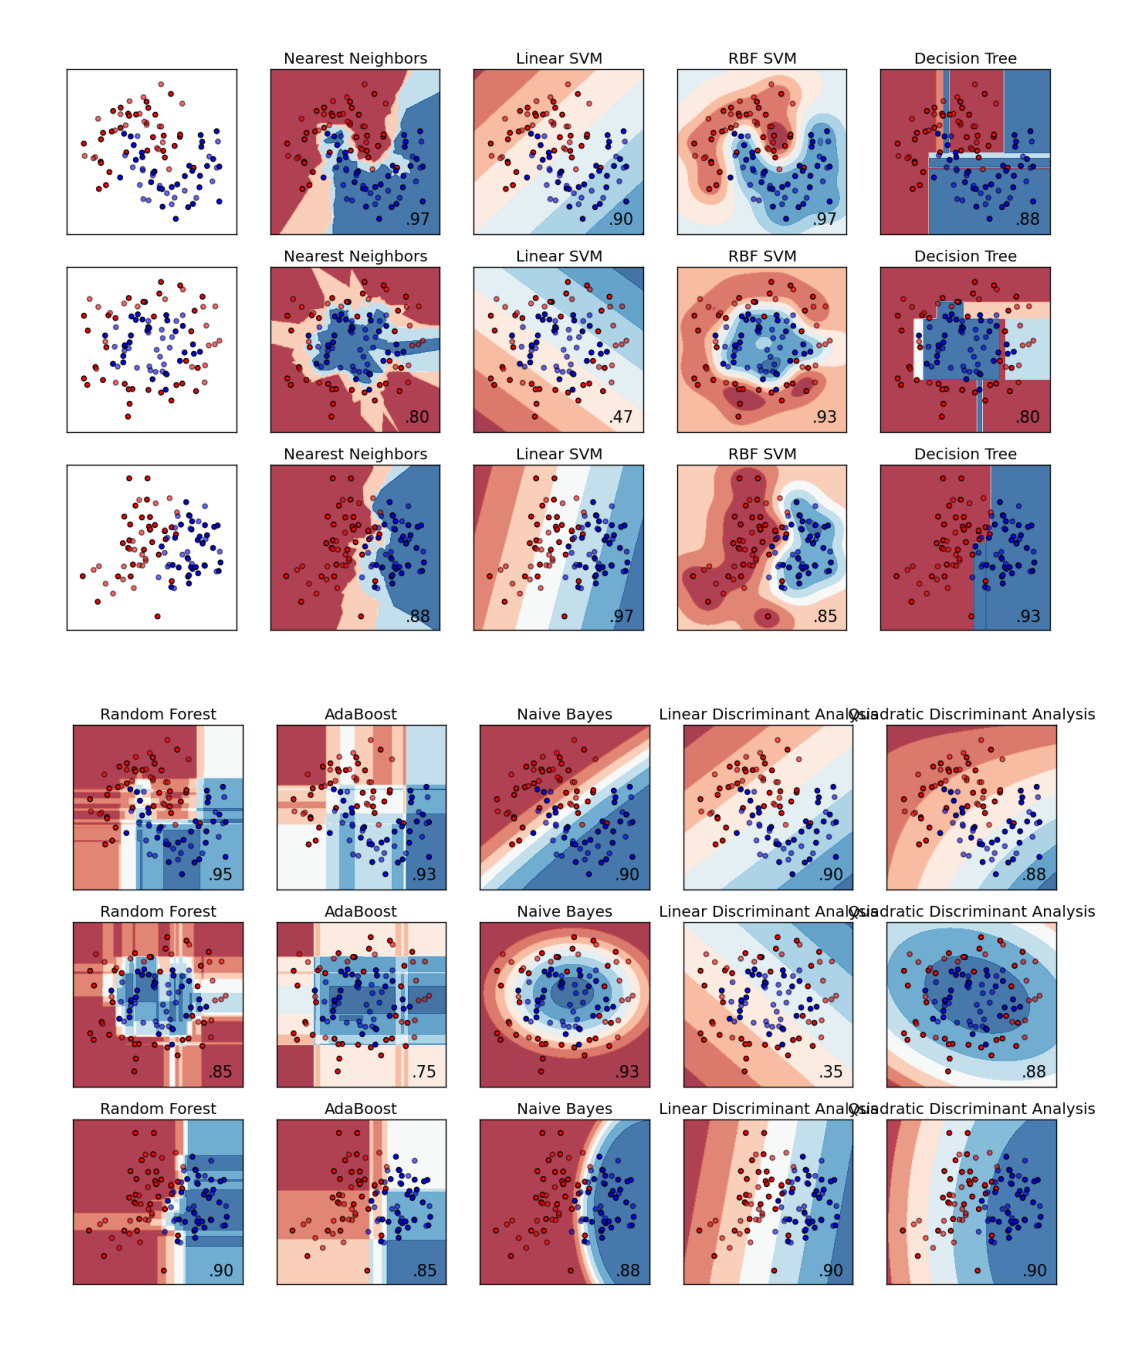
\includegraphics[width=0.9\textwidth]{Figuras/Clasificacion}
      \caption{Ejemplos de clasificación y regresión.[cita]}
    \label{fig:clasificacion}
\end{figure}
 
%http://scikit-learn.org/stable/auto_examples/classification/plot_classifier_comparison.html

\subsubsection{Análisis de Reglas Asociativas}
El análisis de reglas asociativas busca descubrir patrones o asociaciones en base a diferentes elementos en un conjunto de datos. El ejemplo más común de este análisis es el de los carritos de compras en un supermercado. El objetivo en este caso es buscar el patrón de compras conjuntas, por ejemplo, y se puede encontrar un patrón común $\{\textrm{Hamburguesa, Pan}\} \to \textrm{Ketchup}$, es decir, en general las personas que llevan hamburguesa y pan de hamburguesa en el carrito de compra, es probable que también lleven ketchup. 

\begin{figure}[H]
  \centering
    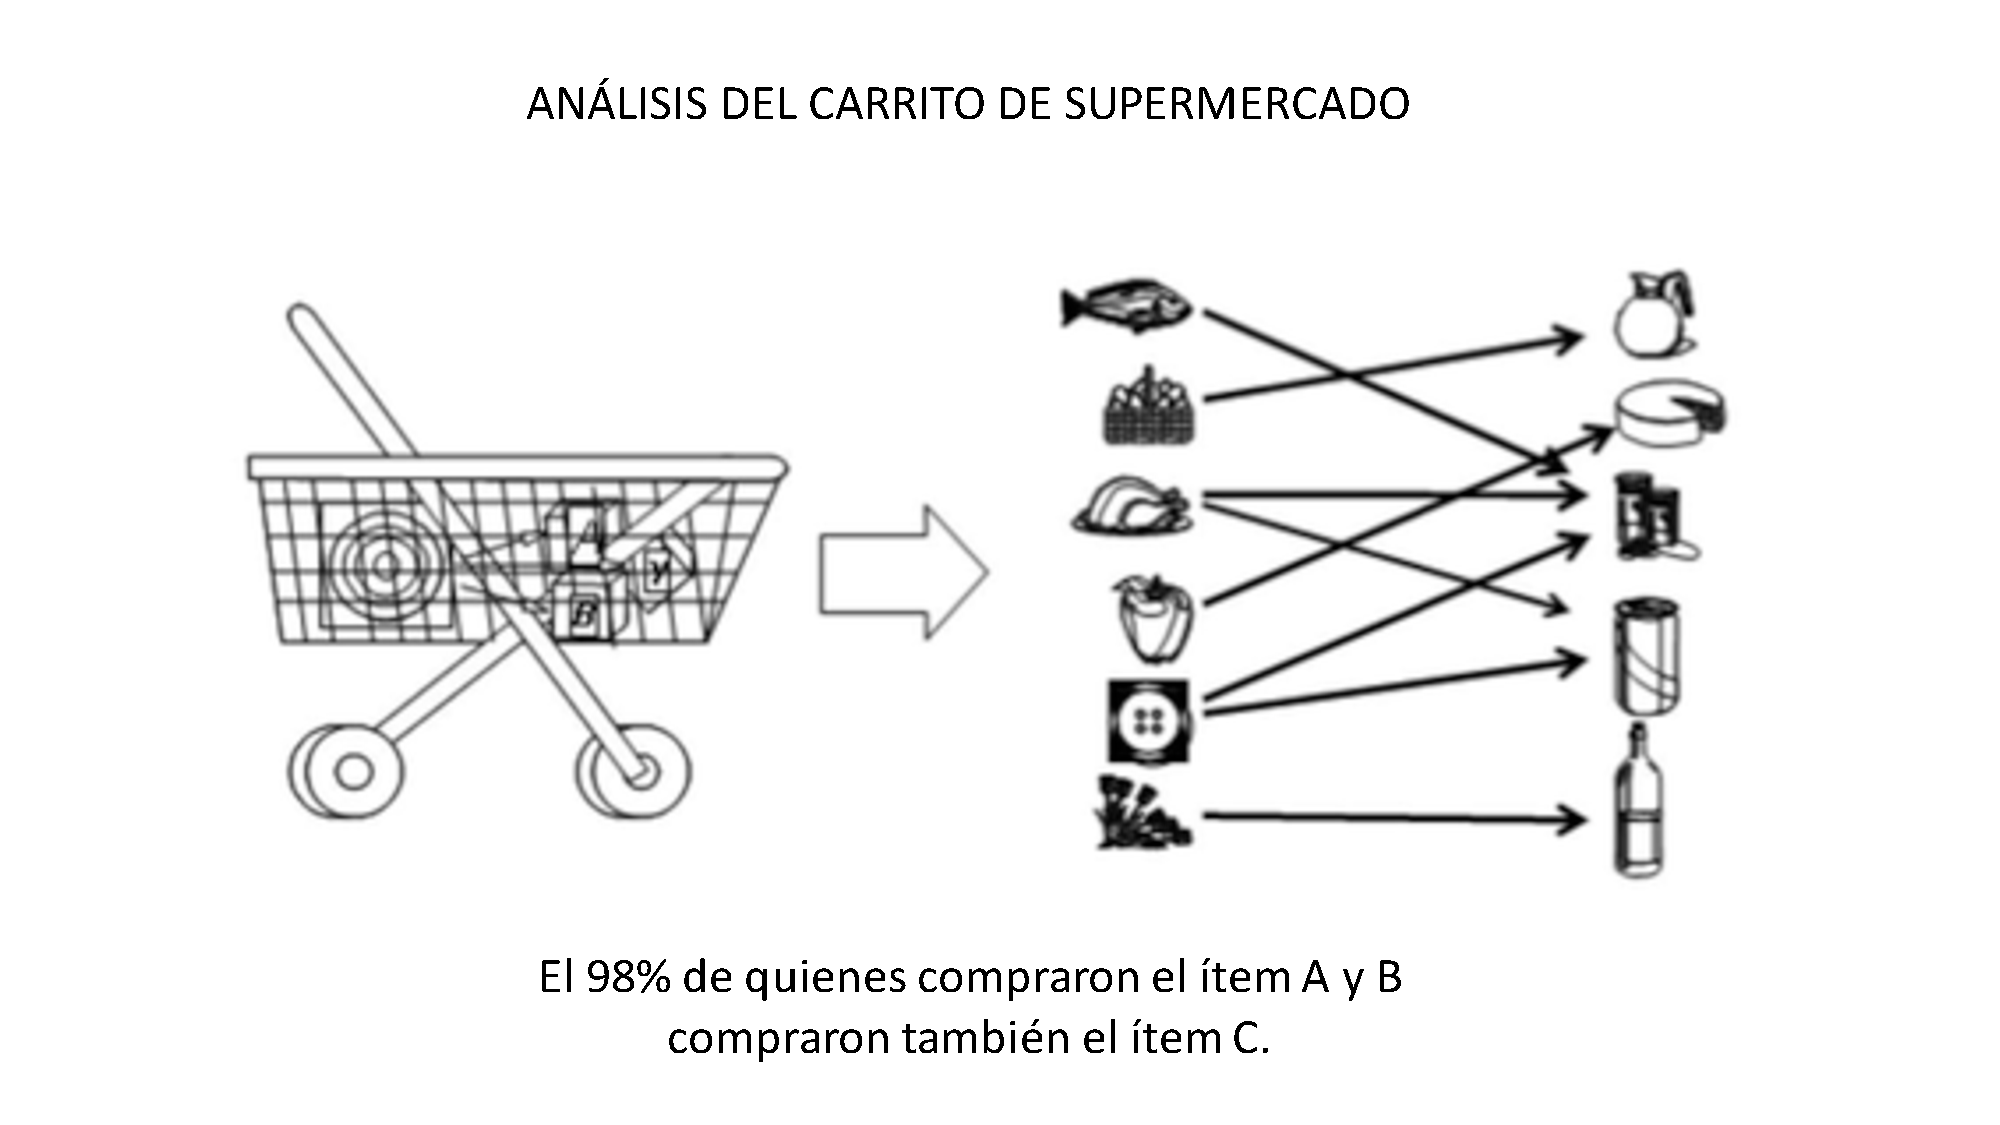
\includegraphics[width=0.7\textwidth]{Figuras/Carrito}
      \caption{Ejemplo del análisis del carrito de supermercado. [cita]}
    \label{fig:carrito}
\end{figure}

En la Figura~\ref{fig:carrito} se puede ver el ejemplo del carrito de supermercados de forma genérica, es decir, se ve representado el patrón de compras, donde el 98\% de los clientes que compraron el ítem A y B, también compraron el ítem C. 

\subsubsection{Análisis de Conglomerados}
Este análisis tiene como objetivo agrupar variables similares en un mismo conglomerado. Las aplicaciones de esto pueden ser la agrupación de documentos de noticias en base al uso de un buscador.

Matemáticamente podemos ver lo siguiente:\\
Teniendo $N$ observaciones con variables $x_1, x_2, x_3, ... , x_i$ se buscan agrupar estas variables en $M$ conglomerados en base a las $N$ observaciones de cada variable. Este método se puede aplicar tanto como a las observaciones o variables.

\begin{figure}[H]
  \centering
    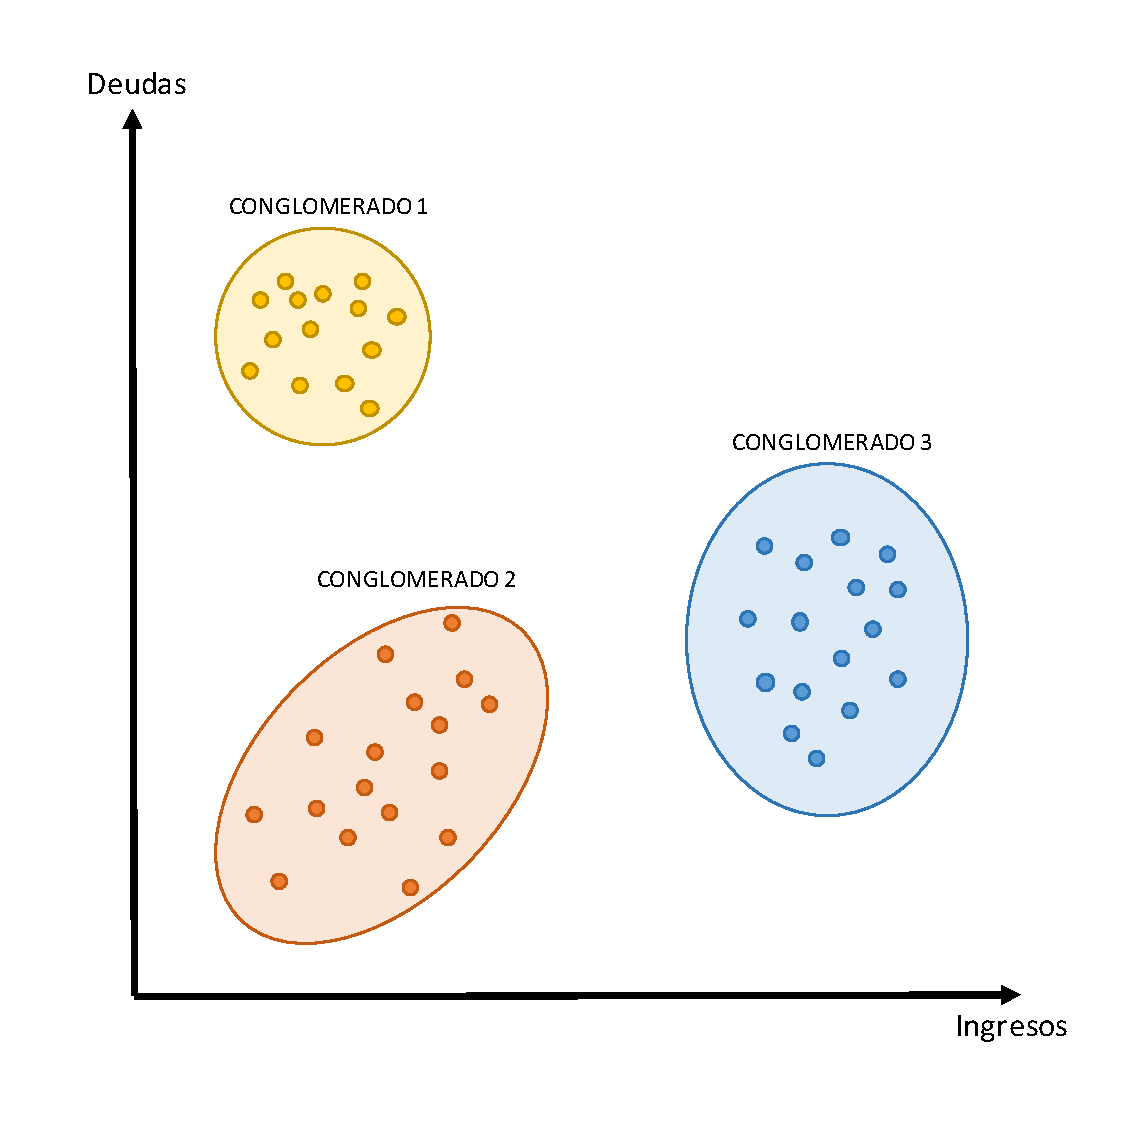
\includegraphics[width=0.9\textwidth]{Figuras/Conglomerados}
      \caption{Ejemplo de análisis de conglomerados.}
    \label{fig:conglomerado}
\end{figure}

Lo que se observa gráficamente en un análisis de conglomerados se muestra en la Figura~\ref{fig:conglomerado}, donde es posible ver que se generan grupos donde sus elementos sean lo más homogéneos posible, y los grupos entre ellos sean lo más heterogéneos posible. 

%[revisar] http://eprints.iisc.ernet.in/273/1/p264-jain.pdf

\subsection{Transformación de los Datos}
La transformación de datos debe estar presente cuando se quiere aplicar minería de datos, ya que es un paso fundamental para que los datos sean legibles y válidos para los algoritmos del procedimiento del modelamiento.

Los procedimientos utilizados en esta etapa son los siguientes:

\begin{description}
  \item[Agrupación de Datos]
  Cuando se tiene muchos datos a veces resulta útil agruparlos para lograr una reducción de estos mejorando su calidad.
  \item[Estructuración de Datos]
  Hay veces donde los datos no  vienen estructurados de la misma forma o simplemente no hay estructura dada. para poder realizar un trabajo de minería de datos es necesario tener un estándar en la estructura de los datos. Por ejemplo, cuando se obtiene información de una página web, esta generalmente no posee una estructura dada, sino que, hay que crearle una para que sea legible y si se tienen más fuentes de datos, es necesario unificar la estructura en una sola.
  \item[Normalización y Discretización de Datos]
  Para que el modelamiento entregue resultados coherentes con la realidad, es sumamente necesario normalizar, discretizar y vectorizar los datos.\\
  La normalización es un procedimiento donde se modifica la escala de los datos logrando que todos tengan una escala de magnitudes similares donde la distancia representará la información y no la magnitud. Generalmente se normaliza utilizando el siguiente procedimiento matemático:
  [formula]
  
  Otra forma de normalizar, que más bien se habla de escalamiento, es utilizando una escala uniforme establecimiento el mínimo y el máximo en la escala. Matemáticamente se puede ver lo siguiente:
  [formula]
  
  Finalmente la discretización y vectorización de los datos implica el uso de algoritmos que son capaces de manejar datos que no poseen magnitud, es decir, categorías para transformarlos en algo numérico que sea legible para el modelo.
  
  La discretización es un procedimiento que lo hace es asignarle números a las categorías, es decir, si tenemos una variable que contiene las siguientes categorías $\{\textrm{Santiago, La Florida, Lo Espejo}\}$ el algoritmo transformará está información en $\{1,2,3\}$. 
  
  La vectorización es también un procedimiento para transformar categorías, pero es aún más útil, puesto que separa cada categoría en una nueva variable donde se señala si se presenta o no cierta categoría. Utilizando el ejemplo anterior donde tenemos una variable categórica con las siguientes categorías $\{\textrm{Santiago, La Florida, Lo Espejo}\}$, al realizar la vectorización, el algoritmo como se puede ver en la Figura~\ref{fig:vect} crea 3 variables dónde cada una indica si la observación es de Santiago, La Florida ó Lo Espejo de forma separada, dónde $1$ señala que presenta esa característica y $0$ cuando no la presenta.
    \begin{table}[H]
    \centering
    \begin{tabular}{l|c|c|c|}
    \cline{2-4}
     & \multicolumn{1}{l|}{\textbf{SANTIAGO}} & \multicolumn{1}{l|}{\textbf{LA FLORIDA}} & \multicolumn{1}{l|}{\textbf{LO ESPEJO}} \\ \hline
    \multicolumn{1}{|l|}{Observación 1} & \textbf{1} & 0 & 0 \\ \hline
    \multicolumn{1}{|l|}{Observación 2} & 0 & \textbf{1} & 0 \\ \hline
    \multicolumn{1}{|l|}{Observación 3} & 0 & 0 & \textbf{1} \\ \hline
    \end{tabular}
    \caption{Ejemplo de una vectorización de variables categóricas}
    \label{fig:vect}
    \end{table}
      
  Todo esto se utiliza por que normalmente los algoritmos de aprendizaje automático requieren el uso de variables numéricas donde la distancia entre los datos es la que se compara, por tanto, no tendría sentido utilizar variables categóricas de texto ni tampoco usar dos variables que tengan diferentes escalas, puesto que los resultados entregados por este estarían influenciados por la variable que tenga la escala más grande.\footnote{Existen métodos que automáticamente manejan estos conflictos. Se hablará de estos más adelante.}

\end{description}
La importancia de este proceso se puede resumir en tres puntos:
\begin{enumerate}
  \item Los datos se obtienen del mundo real donde puede estar incompleta, con ruido y ser inconsistente
  \item La preparación de datos genera un conjunto de datos más pequeño que el original logrando menos tiempo de procesamiento en el proceso del modelamiento
  \item La preparación de datos genera conjuntos de datos de calidad mejorando los patrones encontrados
\end{enumerate}
[cita]
%http://www.cs.ccsu.edu/~markov/ccsu_courses/datamining-3.html

\subsection{Algoritmos de Aprendizaje Automatizado}
Para poder obtener información de los datos, se necesita analizar la información. Lamentablemente cuando tenemos demasiados datos, es imposible obtener información de forma rápida. Debido a esto, se plantearon diferentes algoritmos que buscan automáticamente lo relevante de los datos.
A continuación señalaremos y haremos un breve resumen de los algoritmos más utilizados para la minería de datos.

%http://www.uru.edu/fondoeditorial/libros/pdf/manualdestatistix/cap10.pdf [regresión logística]

\begin{enumerate}
  \item Clasificación y Regresión
    \begin{description}
      \item[Regresión Lineal Simple ó Múltiple] \hfill \\
      El método de regresión lineal tiene como objetivo modelar la relación entre una variable independiente ($y$) y una o más variables dependientes ($x_1, x_2, x_3,...,x_n$). Para modelar esta relación se genera una ecuación de la forma 
      \begin{equation}\label{rlineal}
      y= b_o + b_1 x_1 + b_2 x_2 + ... + b_n x_n 
      \end{equation}
      Donde $b_o,b_1,...,b_n$ son coeficientes escogidos de forma que la suma de cuadrados entre los valores observados y los pronosticados sea mínima, es decir, que se va a minimizar la varianza residual.
      
      Para determinar qué tan buena es una regresión, es decir, cuán precisa es la recta con respecto a los datos, se define el coeficiente de determinación $R^2$. Se trata de un indicador estandarizado que toma valores entre 0 y 1, y da a conocer el porcentaje de datos que son explicados por la regresión. 
      
      En la Figura~\ref{fig:dispersion} se ve un ejemplo de un diagrama de dispersión, donde se muestra el porcentaje de alcohol que contienen diferentes productos y sus precios. Junto a esto, se muestra también la recta de regresión lineal simple, representada por la ecuación $y=20,16+11,61x$, donde $y$ representa el precio y $x$ el porcentaje de alcohol. 
      
    \begin{figure}[H]
        \centering
        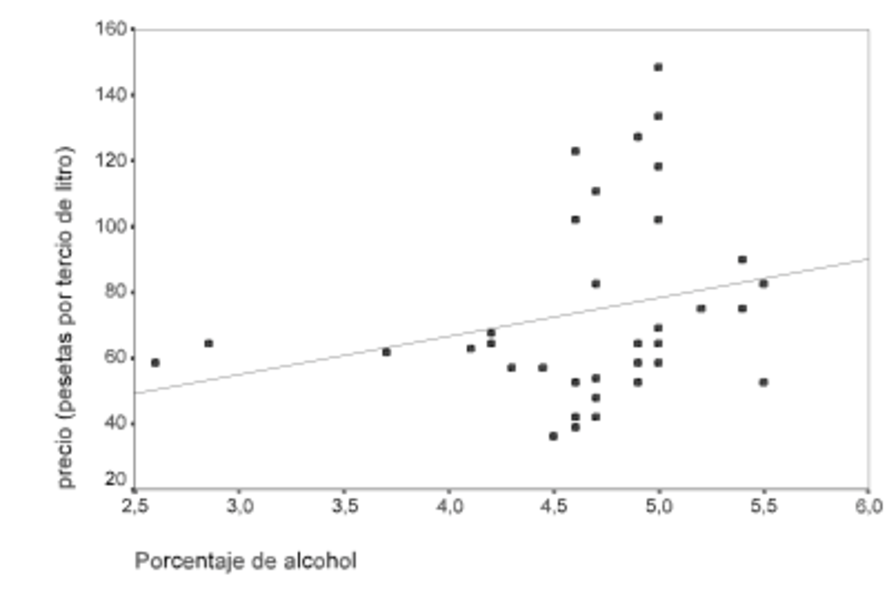
\includegraphics[width=0.7\textwidth]{Figuras/Dispersion}
         \caption{Ejemplo: porcentaje de de alcohol por precio. [cita]}
         \label{fig:dispersion}
    \end{figure}
      
      %http://pendientedemigracion.ucm.es/info/socivmyt/paginas/D_departamento/materiales/analisis_datosyMultivariable/18reglin_SPSS.pdf
      
      Para el ejemplo de la Figura~\ref{fig:dispersion}, $R^2=0,06$ lo que significa que el porcentaje de alcohol contenido en los productos explica sólo el 6\% de su precio. 
      
      \item[Regresión Logística] \hfill \\
      El método de regresión logística es un modelo de regresión lineal en el cual la o las variables dependientes son binarias\footnote{Una variable binaria es aquella que adopta sólo dos valores posibles, como por ejemplo  éxito y fracaso, positivo y negativo, muerto y vivo, buen y mal desempeño,, aprobado o no aprobado.}
      La finalidad de este método de regresión es explicar y predecir una variable categórica binaria\footnote{Las variables categóricas también se denominan variables cualitativas o variables de atributos. Una variable categórica binaria cuenta con dos atributos posibles.}.
      
      Este método es útil para modelar la probabilidad de un evento ocurriendo como función de otros factores.
      
      Se define 
      \begin{equation}
      Odds Ratio = \frac{p}{(1-p)}
      \end{equation}
     Donde $p$ representa la probabilidad de éxito. 
     
     Luego, el modelo logístico se basa en el logaritmo natural de este cociente. 
     
     \begin{equation}
     ln(\frac{p}{(1-p)}) = b_o + b_1 x_1 + b_2 x_2 + ... + b_n x_n 
     \end{equation}
     
     El modelo tiene una formulación equivalente dada por
     \begin{equation}\label{rlogist}
     p=\frac{1}{1-e^-(b_o + b_1 x_1 + b_2 x_2 + ... + b_n x_n)}
     \end{equation}
     
     Gráficamente, la Ecuación~\ref{rlogist} se puede ver en la Figura~\ref{fig:curvalog}, donde $y=1/(1+e^-z); z=b_o + b_1 x_1 + b_2 x_2 + ... + b_n x_n$. Entonces, 
    \begin{itemize}
    \item si $z=0$ entonces $y=0.5$
    \item si $z$ tiende a $+\infty$, entonces  $y=1$
    \item si $z$ tiende a $-\infty$, entonces  $y=0$
    \end{itemize}
     
     
      \begin{figure}[H]
        \centering
        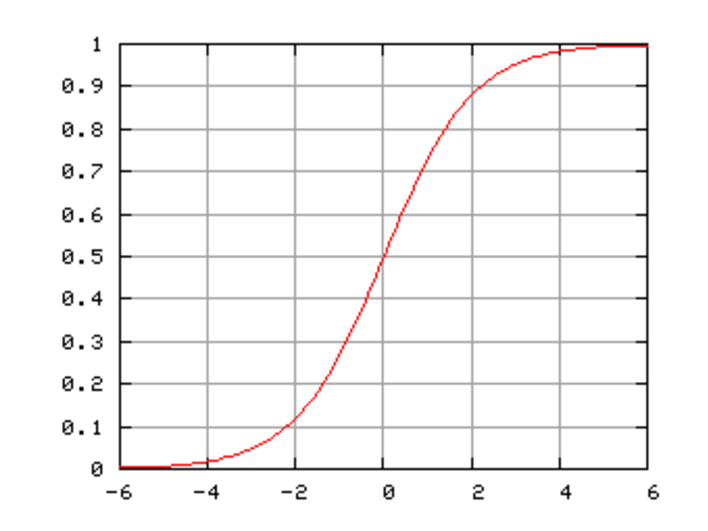
\includegraphics[width=0.7\textwidth]{Figuras/CurvaLog}
         \caption{Curva logística. [cita]}
         \label{fig:curvalog}
    \end{figure}
    %https://es.wikipedia.org/wiki/Función_log%C3%ADstica???? wikipedia????
     
      \item[Máquina de Vectores de Soporte] \hfill \\
      %http://revistas.utp.edu.co/index.php/revistaciencia/article/view/6895/4139
      
      La máquina de vectores de soporte (SVM) es un conjunto de algoritmos de aprendizaje supervisado, es decir, una técnica de predicción. 
      
      Una SVM comienza mapeando los puntos de entrada a un espacio de características de una dimensión mayor, es decir, si los datos se encuentran en $R^2$, son mapeados por la SVM a $R^3$ para encontrar un hiperplano capaz de separarlos en clases y maximizar el margen $m$ entre estas, como se muestra en la Figura~\ref{fig:svm}.
      
      \begin{figure}[H]
        \centering
        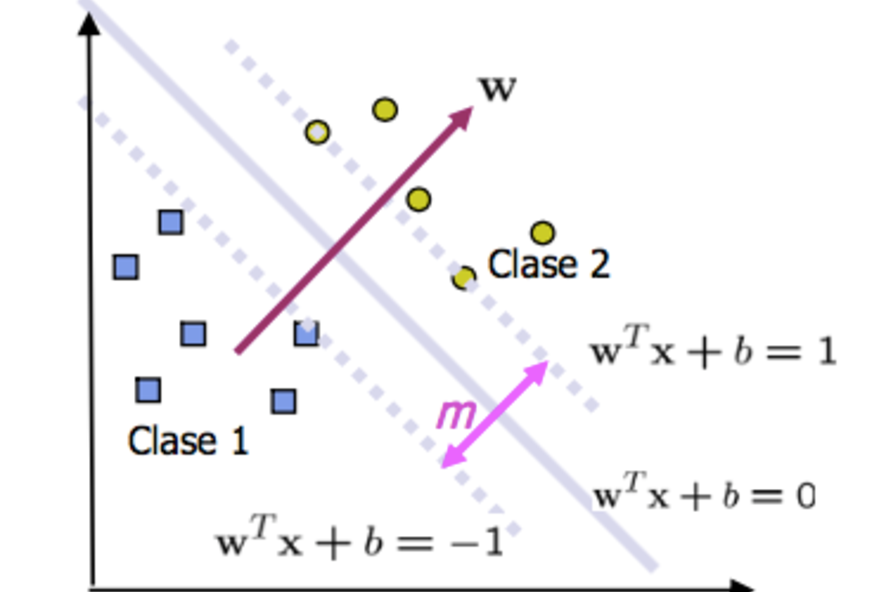
\includegraphics[width=0.7\textwidth]{Figuras/SVM}
         \caption{La frontera de desición debe estar tan lejos de los datos de ambas clases como sea posible. [cita]}
         \label{fig:svm}
      \end{figure}
      
      Entonces, el objetivo es maximizar el margen $m$, lo que se transforma en un problema de programación cuadrática y puede ser resuelto por su problema dual\footnote{Todo problema matemático de programación lineal, conocido como el primal, tiene un dual. Es una definición matemática estrechamente relacionada que se deriva del problema primal. Se define dependiendo del sentido de optimización (maximización o minimización), de los tipos de restricciones (> , < , =) y del signo de las variables (no negativas y no restringidas).} introduciendo multiplicadores de Lagrange\footnote{En los problemas de optimización, el método de los multiplicadores de Lagrange es un procedimiento para encontrar los máximos y mínimos de funciones de múltiples variables sujetas a restricciones mediante derivadas parciales y la regla de la cadena.}. 
      
      Sin ningún tipo de conocimiento del mapeo, la SVM es capaz de encontrar el hiperplano óptimo utilizando el producto punto\footnote{El producto punto de dos vectores es un número real que resulta al multiplicar el producto de sus módulos por el coseno del ángulo que forman.} con funciones en el espacio de características, llamadas kernels. De esta forma, la solución de este hiperplano óptimo puede ser definida a partir de la combinación de unos pocos puntos de entrada, que son los llamados vectores de soporte. 
      
      \item[Naive-Bayes] \hfill \\
      % http://www.researchgate.net/profile/Irina_Rish/publication/228845263_An_empirical_study_of_the_naive_Bayes_classifier/links/00b7d52dc3ccd8d692000000.pdf
      % https://ccc.inaoep.mx/~emorales/Cursos/NvoAprend/bayesiano.pdf
      % http://pages.cs.wisc.edu/~jerryzhu/cs769/nb.pdf
      % http://algoritmosmineriadatos.blogspot.cl/2009/12/algoritmo-naive-bayes.html
      
      El método de Naive Bayes o Clasificador Bayesiano Ingenuo es una técnica de clasificación y predicción supervisada que construye modelos cuyo objetivo es predecir la probabilidad de posibles resultados.
      
      Es un método que simplifica el aprendizaje mediante el supuesto de que las características pertenecen a clases independientes. Aunque la independencia es generalmente una mala suposición, este ingenuo método suele competir bien  clasificadores más sofisticados.
      
      Se basa en el teorema de Bayes, o de la probabilidad condicionada: 
      \begin{equation}\label{bayes}
      P(A|B)=\frac{P(B|A) P(A)}{P(B)}
      \end{equation}
      
      La Ecuación~\ref{bayes} da a conocer el teorema de Bayes, el cual permite conocer la probabilidad de que ocurra el suceso $A$ dado $B$. El supuesto de este teorema es que los sucesos A y B son dependientes, es decir, la probabilidad de que alguno de ellos ocurra está influenciada por la previa ocurrencia del otro.
      
      La forma en que este clasificador trabaja es la siguiente. Como se mencionó anteriormente, este es un método de clasificación probabilístico, que será utilizado para clasificar un nuevo elemento $X$, definido como un vector $X=(X_1, X_2, ..., X_n)$, dentro de un conjunto finito $C={C_1, C_2, ..., C_n}$ de clases determinadas. Esto significa que, dada una clase $C$, se calcula la probabilidad de que dicho elemento se clasifique dentro de la categoría $C$, como lo muestra la Ecuación~\ref{pclase}, donde $P(C)$ es la probabilidad a priori de la clase, $P(X|C)$ es la probabilidad condicional del elemento $X$ dada la clase $C$.
      \begin{equation}\label{pclase}
      P(C|X)=\frac{P(X|C) P(C)}{P(X)}
      \end{equation}
      
      En base a los datos observados, la probabilidad de que cada uno pertenezca a cada clase es conocida, y la probabilidad de cada clase también. Por lo que lo que necesita encontrar es el máximo valor de la expresión para encontrar la clase que mejor clasifica al nuevo elemento $X$. 
      
      El nuevo elemento $X$ a clasificar se encuentra definido en términos del vector $X=(X_1, X_2, ..., X_n)$. Además, existe un conjunto finito de clases $C={C_1, C_2, ..., C_n}$ en las que puede ser clasificado dicho vector. Finalmente, el método Naive Bayes clasifica el elemento $X$ en una de todas las clases existentes utilizando la Ecuación~\ref{mclase}.

      \begin{equation}\label{mclase}
      Mejor Clase = Argmax_{c_j\in C} P(c_j) \prod P(x_i|c_j)
      \end{equation}
      
      \item[Redes Neuronales] \hfill \\
      %http://citeseerx.ist.psu.edu/viewdoc/download?doi=10.1.1.125.4567&rep=rep1&type=pdf
      %http://avellano.fis.usal.es/~lalonso/compt_soft/articulos/dataminingnn.pdf
    
      Las redes neuronales son conexiones de nodos conectados, con entradas,  salidas y procesamiento en cada nodo. Entre las entradas y salidas de una red neuronal existen capas ocultas de procesamiento, tal como es posible observar en la Figura~\ref{fig:redneuronal}, la cual presenta su capa de salida, que es lo que se quiere predecir, una capa oculta cuyo objetivo es transformar el espacio de entrada en otro más propicio para que las neuronas de salida puedan realizar discriminaciones lineales, y una capa de entrada que representan los atributos con los que se quiere realizar la predicción. 
      
      Una red neuronal debe ser entrenada con un conjunto de patrones de entrenamiento (aprendizaje supervisado). Una vez entrenada, es capaz de realizar predicciones. 
      
       \begin{figure}[H]
        \centering
        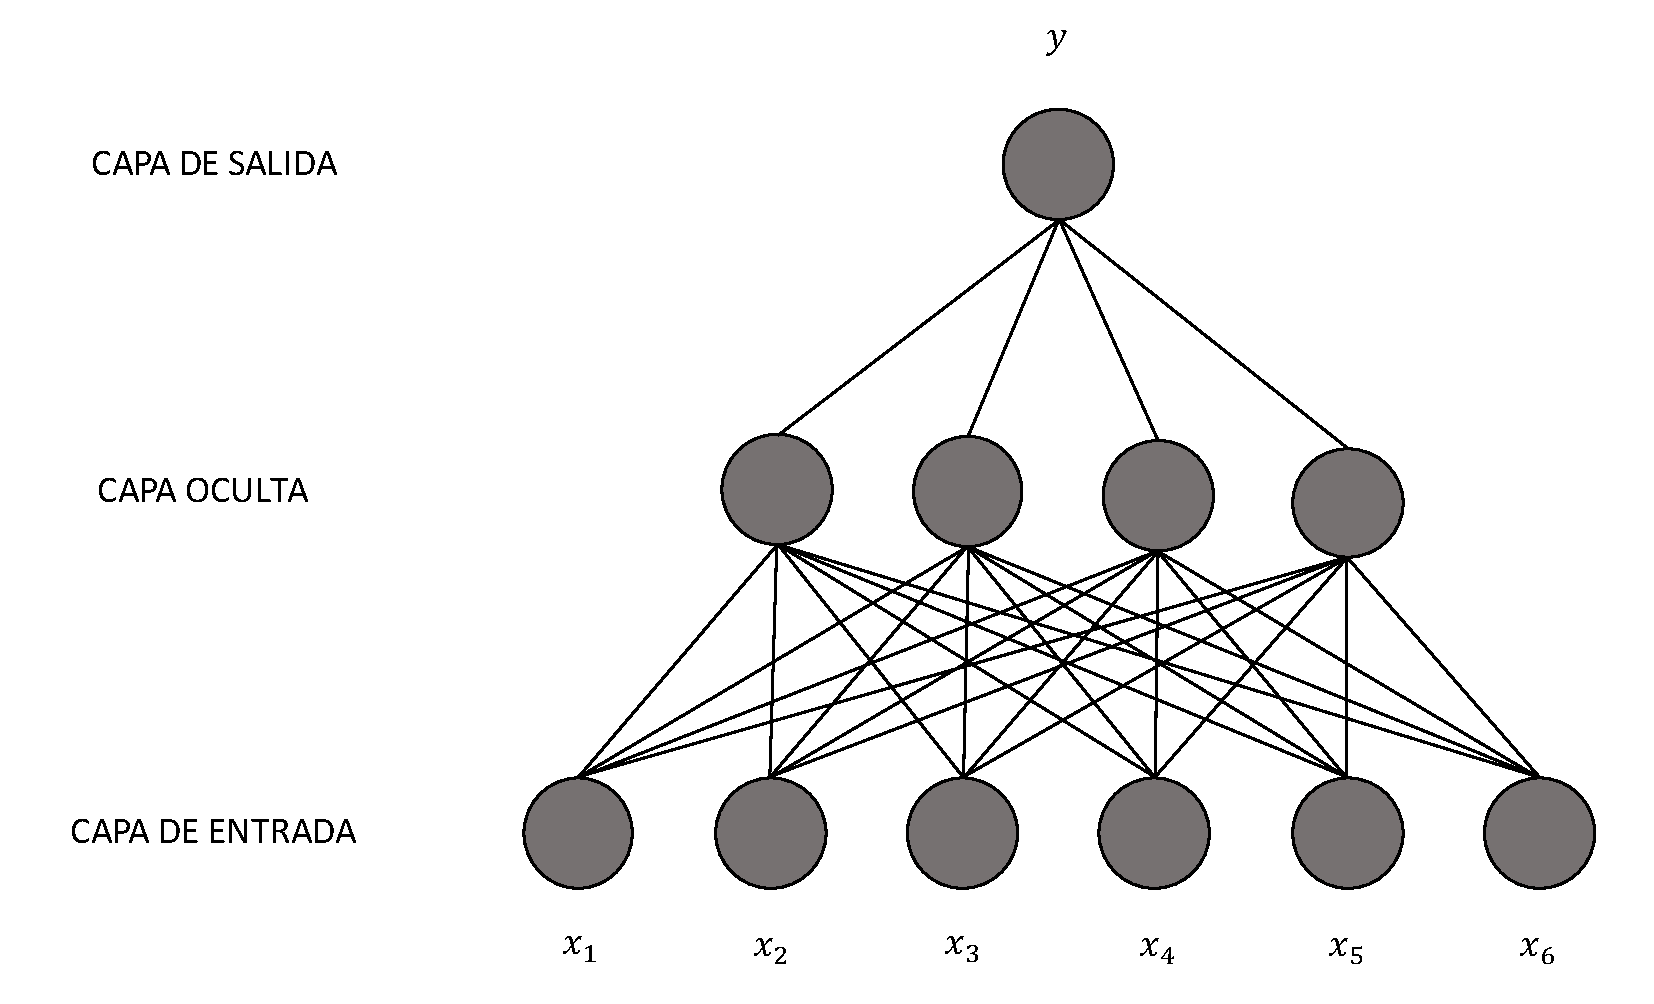
\includegraphics[width=0.7\textwidth]{Figuras/RedNeuronal}
         \caption{Vista gráfica de una red neuronal.  [cita]}
         \label{fig:redneuronal}
      \end{figure}
      %http://materias.fi.uba.ar/7500/bot-tesisdegradoingenieriainformatica.pdf

      \item[Vecino Más Cercano] \hfill \\
     %http://citeseerx.ist.psu.edu/viewdoc/download?doi=10.1.1.220.2882&rep=rep1&type=pdf
     
     El método del vecino más cercano es uno de los métodos de clasificación más simples de los algoritmos para la predicción de clases. Este se basa en el aprendizaje supervisado, es decir, en la existencia de dos muestras: una de entrenamiento y otra de testeo. Gracias a la muestra de entrenamiento, que contiene casos ($x$) con sus respectivas etiquetas ($y$), posible hacer la predicción para los casos de la muestra de testeo.
     
     Específicamente, este método lo que hace es, dado un conjunto de datos de la forma $(x,y)$, transformarlos en una función de distancia. 
     
     Este método básico se llama el algoritmo kNN. Hay dos principales opciones de diseño para hacer: el valor de k, y la función de distancia para su uso. Cuando hay dos clases alternativas, con el fin de evitar lazos la elección más común para k es un pequeño entero impar, por ejemplo k = 3. Si hay más de dos clases, a continuación, los lazos son posibles incluso cuando k es impar. Lazos también pueden surgir cuando dos valores de distancia son lo mismo. Una implementación de kNN necesita un algoritmo razonable para romper los lazos; no existe un consenso sobre la mejor manera de hacer esto.
     
     Cuando cada ejemplo es un vector de longitud fija de números reales, la función de distancia más común es la distancia euclídea, que se muestra en la Ecuación~\ref{distancia}.
     \begin{equation}\label{distancia}
     d(x,y)=||x-y||=\sqrt{(x-y) \cdot (x-y)}=(\sum_{i=1}^m (x_i - y_i )^2)^{1/2}
     \end{equation}
      Donde $x$ e $y$ son puntos en $X=\mathsf{R}^m$.
      
      \item[Árboles de Decisión] \hfill \\
      %http://dmle.cindoc.csic.es/pdf/QUESTIIO_2001_25_03_04.pdf
      %
      
      Los árboles de decisión son un método de clasificación, y tal como lo dice su nombre, su uso permite clasificar elementos a partir de los atributos de cada elemento. 
      
      Por lo que la forma en que este método actúa es predijendo el valor de una variable de destino $y$ a partir de diversas variables de entrada $x_i$.
      
      En la Figura~\ref{fig:arbol} es posible observar gráficamente un árbol de decisión, donde cada nodo interior corresponde a una de las variables de entrada, cada hoja representa un valor de la variable de destino dados los valores de las variables de entrada representados por el camino desde la raíz a la hoja.
      
      \begin{figure}[H]
        \centering
        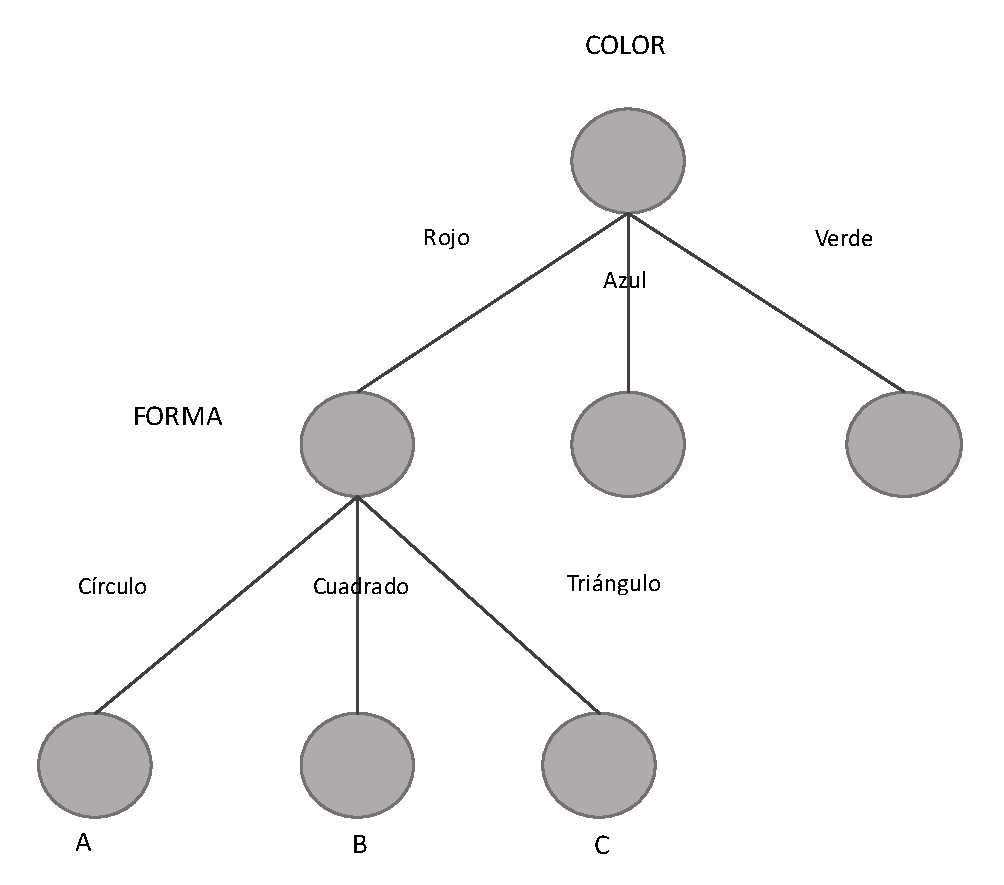
\includegraphics[width=0.7\textwidth]{Figuras/Arbol}
         \caption{Vista gráfica de un árbol de decisión.}
         \label{fig:arbol}
      \end{figure}
      
      Por ejemplo, si un dato posee los atributos color=rojo y forma=cuadrado, sería clasificado en la categoría B, como se muestra en la Figura~\ref{fig:arbol}. 
      
      \item[Bosques Aleatorios] \hfill \\
      %http://machinelearning202.pbworks.com/w/file/fetch/60606349/breiman_randomforests.pdf
      
      Los bosques aleatorios son un método de clasificación y predicción que consiste en la combinación de árboles de de decisión, en la que cada árbol depende de los valores de un vector aleatorio probado independientemente y con la misma distribución para cada uno de estos.
      
      Este es un algoritmo que mejora la precisión en la clasificación mediante la incorporación de aleatoriedad en la construcción de cada clasificador individual. Esta aleatorización puede introducirse tanto en la partición del espacio (construcción del árbol), así como en la muestra de entrenamiento. Los bosques aleatorios comienzan con una técnica de aprendizaje automático estándar descrita anteriormente, árbol de decisión, que, en cuanto al conjunto, corresponde a un aprendizaje. Tal como fue descrito, en un árbol de decisión, una entrada se introduce en la parte superior y hacia abajo a medida que atraviesa el árbol de los datos, los cuales se acumulan en conjuntos más pequeños.
      
      Este método permite hacer de manera segura predicciones más precisas y sin la mayoría de los errores básicos comunes a otros métodos.
      
      \item[AdaBoost] \hfill \\
      %http://citeseerx.ist.psu.edu/viewdoc/download?doi=10.1.1.9.329&rep=rep1&type=pdf 
      
      El AdaBoost o \textit{Adaptive Boosting} es un método que construye una regla de clasificación final utilizando varios clasificadores menores, denominados “débiles” por su sencillez y escasa precisión. En solitario estos clasificadores débiles no constituirían un sistema de clasificación útil debido a su alta inexactitud, pero al usarlos en conjunto es posible construir un clasificador mucho más preciso. Los clasificadores débiles corresponden a reglas de clasificación simples y que entregan como resultado un valor de confianza, o confidencia, respecto a la predicción que están haciendo.
      
      Los clasificadores débiles  generan resultados pobres, pero es posible  definir clasificadores mas robustos enlazando una serie de módulos como el de la figura,  incrementando de manera exponencial el éxito de detección. Aun cuando estos clasificadores fuertes  pueden llegar a una tasa de detección del 99\%, la tasa de falsos positivos puede ubicarse por encima de 30\%.
      
      \item[GradientBoost] \hfill \\
      %https://www.cs.princeton.edu/courses/archive/spring07/cos424/papers/boosting-survey.pdf
      
      \textit{Gradient Boost} es un método de aprendizaje automático para problemas de regresión y clasificación. La idea es generar un modelo de predicción en forma de un conjunto de modelos de predicción débiles, que son, por lo general, árboles de decisión. La forma en que el modelo es construido es mediante etapas, Construye el modelo mediante etapas, y los generaliza, permitiéndoles optimizar de manera arbitraria la función de pérdida.
      
    \end{description}
    
    
  \item Análisis de Reglas Asociativas
    \begin{description}
    
      \item[Apriori] \hfill \\
      The first item
      
      \item[Eclat] \hfill \\
      The second item
      
      \item[FP-Growth] \hfill \\
      The third etc \ldots
      
    \end{description}
    
    
  \item Análisis de Conglomerados
    \begin{description}
    
      \item[Vecino Más Cercano] \hfill \\
      The first item
      
      \item[DBSCAN] \hfill \\
      The second item
      
      \item[K-means] \hfill \\
      The third etc \ldots
      
    \end{description}
\end{enumerate}


\subsection{Validación del Modelo}

Una vez obtenido un modelo, es necesario validar que el modelo es capaz de generalizar para observaciones nuevas. El gran problema que puede ocurrir con un modelo es el sobre-ajuste, es decir, el modelo se ajusta perfectamente a los datos entregados, pero al momento de evaluar datos nuevos, entrega información incorrecta. Esto se puede ver muy fácilmente para una regresión. En el gráfico se ve que el modelo se ajusta muy bien a los datos entregados [grafico], pero no así con los datos nuevos [grafico].Para evitar el sobre-ajuste, es necesario realizar un procedimiento llamado validación cruzada.

La validación de un modelo consta de la división del conjunto de datos entre un conjunto llamado 'conjunto de entrenamiento' y 'conjunto de prueba'. Solamente se entrena el modelo con el conjunto de entrenamiento, mientras que el conjunto de prueba se utiliza para ver el verdadero desempeño del modelo y obteniendo el error de entrenamiento y el error de prueba. El problema de esto es que estos errores no son buenos estimadores del desempeño de la generalización del modelo, puesto que los conjuntos no cambian Para obtener un buen estimador se utiliza la validación cruzada, que, como lo señala su nombre, es lo mismo que la validación, pero se agregan pasos iterativos que van permutando el conjunto de entrenamiento y de prueba para obtener un error promedio que si es representativo del problema.

Existen múltiples métodos de validación cruzadas, a continuación se señalarán algunos:
    \begin{description}
      \item[Hold-out Validation] \hfill \\
      The first item
      [grafico]
      \item[K-fold Cross-Validation] \hfill \\
      The second item
      [grafico]
      \item[Leave-One-Out Cross-Validation] \hfill \\
      The third etc \ldots
      [grafico]
    \end{description}

% Please add the following required packages to your document preamble:
% If you use beamer only pass "xcolor=table" option, i.e. \documentclass[xcolor=table]{beamer}
\begin{table}[H]
\centering
\resizebox{\textwidth}{!}{%
\begin{tabular}{|c|c|c|}
\hline
\rowcolor[HTML]{C0C0C0} 
\textbf{Método de Validación} & \textbf{Pros} & \textbf{Contras} \\ \hline
Validación con restitución & Simple de implementar & Tendencia al sobre-ajuste \\ \hline
Validación con retención & \begin{tabular}[c]{@{}c@{}}Conjunto de entrenamiento y\\  conjunto de prueba independientes\end{tabular} & \begin{tabular}[c]{@{}c@{}}Set de entrenamiento y set de prueba \\ reducidos, varianza grande\end{tabular} \\ \hline
\begin{tabular}[c]{@{}c@{}}Validación cruzada con \\ k-permutaciones\end{tabular} & \begin{tabular}[c]{@{}c@{}}Mayor exactitud de la estimación \\ del desempeño\end{tabular} & \begin{tabular}[c]{@{}c@{}}Muestra pequeña de estimación; \\ Varianza subestimada\end{tabular} \\ \hline
\begin{tabular}[c]{@{}c@{}}Validación cruzada \\ dejando un dato fuera\end{tabular} & \begin{tabular}[c]{@{}c@{}}La estimación del desempeño no está \\  sesgada\end{tabular} & Varianza muy grande \\ \hline
\begin{tabular}[c]{@{}c@{}}Validación cruzada con \\ k-permutaciones repetidas\end{tabular} & Varias estimaciones del desempeño & Varianza subestimada \\ \hline
\end{tabular}
}
\caption{Pros y contras de diferentes métodos de validación.}
\label{mvalidacion}
\end{table}

% [tabla] Cross-Validation. Table 1. Pros and Cons of different validation methods

\subsection{Afinación de los Parámetros del Modelo}
La mayoría de los modelos poseen parámetros que definen diferentes atributos de este. Estos parámetros normalmente se determinan \textit{a priori}. Existen métodos que, en conjunto con la validación cruzada, logran además, encontrar los parámetros que más se acerquen al óptimo. Esto se hace con una técnica llamada Búsqueda Aleatoria de Grilla [cita]. Lo que hace la Búsqueda Aleatoria de Grilla es, a través de una distribución de probabilidad dada, crear una grilla de estos valores e ir probando $N$ valores de forma aleatoria hasta que se acerque al óptimo. En general, siempre se obtiene algo mejor, pero es difícil llegar al óptimo, dado la naturaleza del problema de búsqueda en optimización, donde la limitante para hacer una búsqueda exhaustiva es la capacidad computacional.
[grafico]
\subsection{Medición del Desempeño del Modelo}

Para evaluar el desempeño de un modelo se pueden utilizar diferentes medidas. Para nuestro estudio solamente señalaremos las más importantes que son la precisión y la exhaustividad.La precisión cuando hablamos de una tarea de clasificación se define como la proporción de las observaciones que son clasificados correctamente y la exhaustividad es la proporción de observaciones relevantes correctamente clasificadas.

\begin{figure}[H]
  \centering
    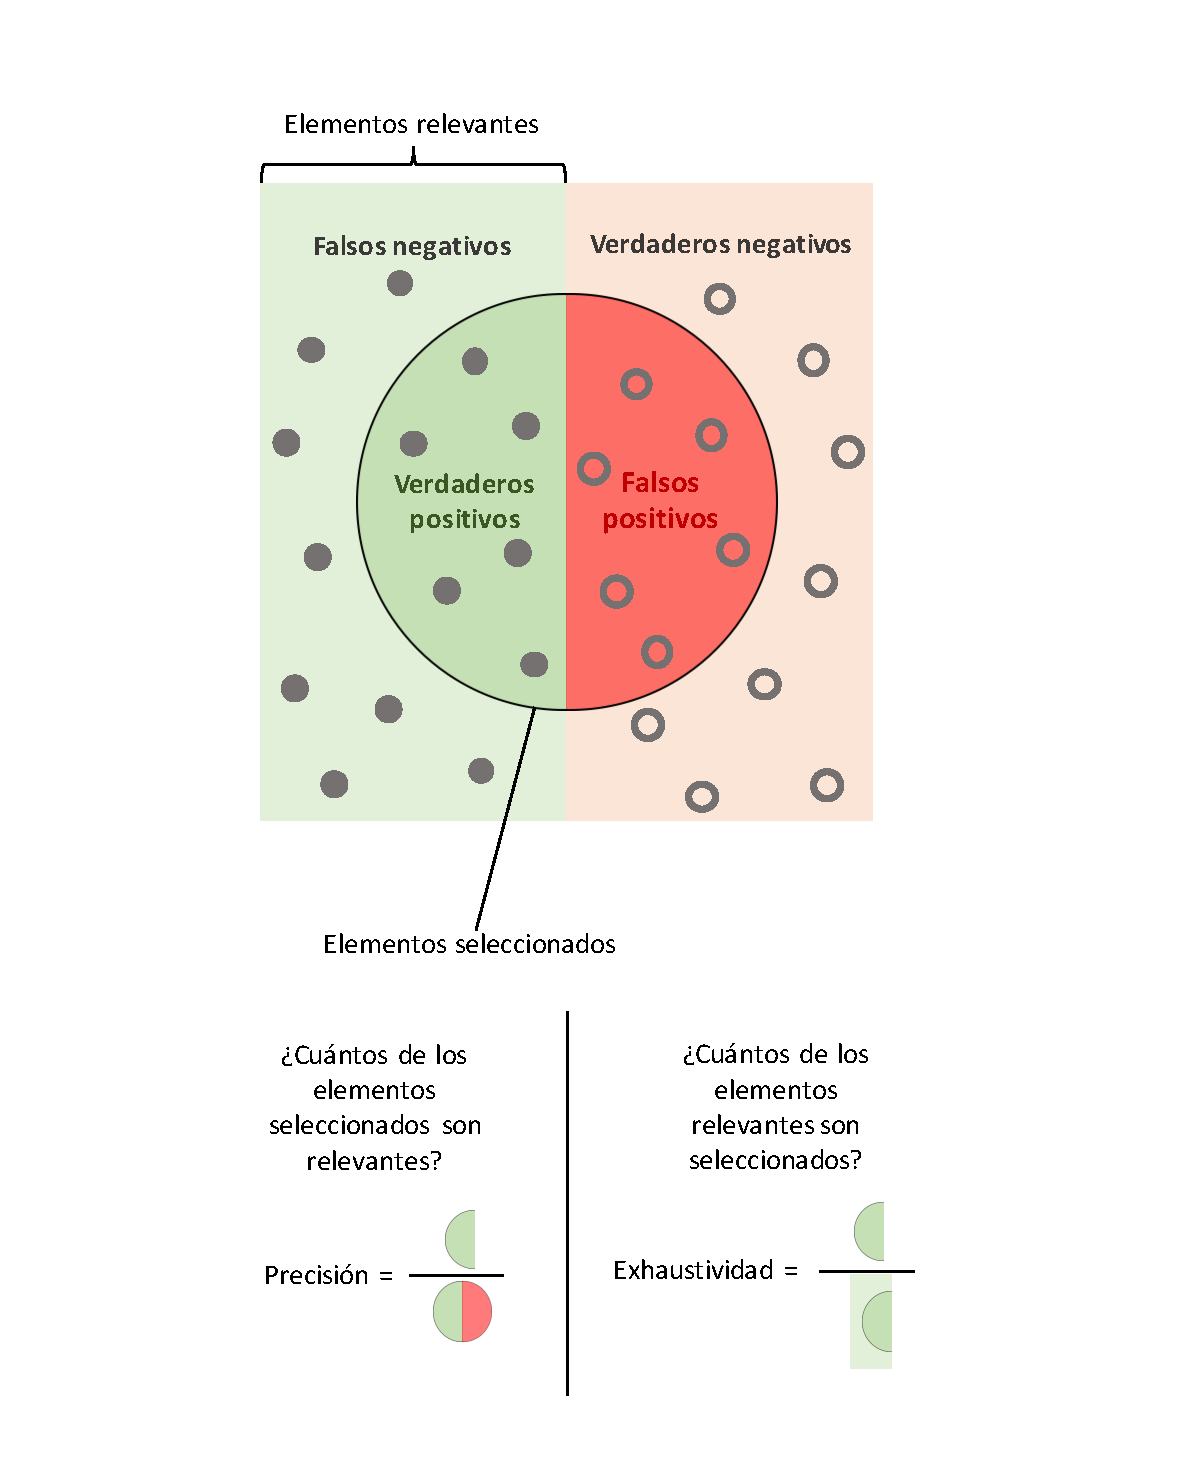
\includegraphics[width=0.9\textwidth]{Figuras/Precision}
      \caption{Descripción gráfica de presición y exhaustividad.}
    \label{fig:precision}
\end{figure}


% https://upload.wikimedia.org/wikipedia/commons/thumb/2/26/Precisionrecall.svg/440px-Precisionrecall.svg.png

Para poder obtener toda esta información debemos, como primer paso, calcular la llamada \textit[matriz de confusión] dónde resume el resultado de la tarea de clasificación.

[grafico] 
%rehacer tabla con colores señalando que es error tipo I y II: https://en.wikipedia.org/wiki/Confusion_matrix

% Please add the following required packages to your document preamble:
% \usepackage{multirow}
\begin{table}[H]
\centering
\begin{tabular}{lc|c|c|}
\cline{3-4}
 & \multicolumn{1}{l|}{} & \multicolumn{2}{c|}{Condición verdadera} \\ \cline{2-4} 
\multicolumn{1}{l|}{} & Población total & Condición positiva & Condición negativa \\ \hline
\multicolumn{1}{|c|}{\multirow{2}{*}{\begin{tabular}[c]{@{}c@{}}Condición\\ de \\ predicción\end{tabular}}} & \begin{tabular}[c]{@{}c@{}}Condición de \\ predicción positiva\end{tabular} & Verdadero positivo & \begin{tabular}[c]{@{}c@{}}Falso positivo\\ (Error tipo I)\end{tabular} \\ \cline{2-4} 
\multicolumn{1}{|c|}{} & \begin{tabular}[c]{@{}c@{}}Condición de \\ predicción negativa\end{tabular} & \begin{tabular}[c]{@{}c@{}}Falso negativo\\ (Error tipo II)\end{tabular} & Verdadero negativo \\ \hline
\end{tabular}
\caption{Matriz de confusión.}
\label{mconfusion}
\end{table}


[cita] 
%http://www.flinders.edu.au/science_engineering/fms/School-CSEM/publications/tech_reps-research_artfcts/TRRA_2007.pdf

\section{Herramientas Computacionales}
Para poder desarrollar este trabajo se deben integrar diferentes herramientas para realizar la transformación, preparación, modelamiento y validación de los datos.
\subsection{Lenguaje de Programación Python}
Python es un lenguaje de programación de alto nivel para resolver todo tipo de problemas. Este soporta programar en diferentes paradigmas y manejo automático del uso de recursos. Además tiene un énfasis en la legibilidad imponiendo un orden en el código.
En general, las ventajas de Python son las siguientes:\\
\begin{itemize}
  \item Intuitivo
  \item Flexible
  \item Comunidad activa
  \item Excelente documentación
\end{itemize}
Python se basa en paquetes o librerías para poder distribuir soluciones especificas, a continuación se nombrarán las que serán utilizadas durante el trabajo.\footnote{Ver más sobre Python: https://www.python.org}
\subsubsection{Librerías}
\begin{description}
  \item[NumPy] \hfill \\
  Libería fundamental para el trabajo cientifico con Python. Se utiliza para trabajar con arreglos multidimensionales, algebra lineal y herramientas para implementar soluciones en lenguajes de bajo nivel(C/C++\footnote{Lenguaje de programación muy utilizado de bajo nivel que logra una rapidez y eficiencia en el uso de recursos.}) para obtener un mejor rendimiento.
  \item[Pandas] \hfill \\
  Manejo de datos de forma estructurada rápidamente y sencilla. Se utiliza mucho para hacer analisis de los datos y posee compatibilidad varias estructuras de información como SQL, CSV y TSV.
  \item[Scikit-Learn] \cite{scikit-learn} \hfill \\
  Implementación de algoritmos de machine learning de forma sencilla e intuitiva.
  \item[Scikit-Learn-NNet] \hfill \\
  Implementación de redes neuronales para la librería scikit-learn.
  \item[Matplotlib] \hfill \\
  Librería de visualización de bajo nivel para realizar diferentes tipos de gráficos 2D.
  \item[Seaborn] \hfill \\
  Libería de visualización basada en matplotlib de alto nivel para poder graficar de forma sencilla.
  \item[IPython] \hfill \\
  Shell interactiva para Python para poder explorar y trabajar en la memoria. Simula el estilo de MatLab y R.
\end{description}
Todas las liberías utilizadas en este proyecto, incluido Python son de código libre y de libertad de uso.
\subsection{PyCharm}
Interfaz de desarrollo para Python basado en Eclipse.\footnote{Ver más sobre PyCharm: https://www.jetbrains.com/pycharm/Py}
\subsection{Tableau}
Herramienta intuitiva de visualización y exploración de datos muy usado en la industria. Tiene gran capacidad de análisis.\footnote{Ver más sobre Tableau: http://www.tableau.com/}
\subsection{Microsoft Excel 2016}
Herramienta para el manejo de hojas de cálculo y datos estructurados de forma sencilla.\footnote{Ver más sobre Excel: https://products.office.com/en-us/excel/}
\subsection{QGIS}
Sistema de información geográfica de código libre para el manejo y análisis de datos con geo-refencia.\footnote{Ver más sobre QGIS: http://www.qgis.org/es/site/}
\section{Conclusiones}

Durante este capitulo se presentaron las herramientas estadísticas y computacionales, junto con la metodología de trabajo que llevaremos a cabo para lograr el objetivo del proyecto. Nos guiaremos por la metodología CRISP-DM dado su amplio uso en la minería de datos y usaremos herramientas potentes de código libre. Se utilizará Python y sus librería para todas las etapas de la metodología y en conjunto con herramientas de visualización potente para las áreas exploratorias y descriptivas que se vayan necesitando. En general este conjunto de herramientas